\subsection{Introduction}

Monte Carlo simulation is the  standard (if not the only) technique for most numerical problems in stochastic modelling.
It has a long history and has been successfully applied in many fields, such as biology~\cite{Manly2018RandomizationBiology}, statistical Physics~\cite{Binder2012MontePhysics}, Finance~\cite{Glasserman1997CounterexamplesProbabilities} among others.
The default order of magnitude for the variance of the estimator is~$\Oo(N^{-1/2})$ with~$N$ the number of sample paths.
It has long been recognised though that several tricks achieve lower variance with equivalent (hopefully zero) bias; among those antithetic variables and importance, sampling have become ubiquitous.
We focus on the latter, for which large and moderate deviations (LDP and MDP) provide closed-form formulae, 
making their applications pain-free and without additional computer costs. For any further details, we refer the reader to the original work~\cite{Geha2023LargeModel}.

The first attempt to reduce the variance of a Monte Carlo estimator based on asymptotics originated, rather heuristically, in~\cite{Siegmund1976ImportanceTests}. 
This was then made rigorous by Glasserman and Wang~\cite{Glasserman1997CounterexamplesProbabilities}, who also highlighted pitfalls of the method and by Dupuis and Wang~\cite{Dupuis2004ImportanceGames}, who provided clear explanations on the trade-off between asymptotic approximations and the restrictions they entail on the induced change of measure.
Guasoni and Robertson~\cite{Guasoni2007OptimalTime} 
put this into practice for out-the-money path-dependent options in the Black-Scholes model,
and Robertson~\cite{Robertson2010SampleModels} developed a thorough analysis for the Heston model using sample path large deviations.
This is our starting point,
and the goal of our current enterprise is to analyse different asymptotic regimes 
(small-time, large-time, small-noise),
both in the large deviations and in the moderate deviations regimes, in the Heston model 
and to show how these yield closed-form formulae for an optimal change of measure for importance sampling purposes.

In~\cite{Geha2023LargeModel} we propose, in particular, a specific form of adaptive drift, allowing for fast computation
and increase in variance reduction.
For  geometric Asian Call options in the Heston model, MDP-based estimators with deterministic changes of drift turn out to be no better than those computed with deterministic volatility approximation in the LDP approach. 
However, MDP-based estimators with adaptive changes of drift perform much better than their LDP counterparts with deterministic volatility approximation, 
and in fact, show a performance very close to the LDP-based estimators in Heston. 
These adaptive MDP-based estimators, therefore, provide an efficient alternative in models where 
LDP is difficult to compute.

\textbf{Setting and notations} Throughout this chapter we work on a filtered probability space~$(\Omega, \Ff, \PP, \FF)$ with a finite time horizon~$T>0$, where~$\Omega = \Cc([0,T]; \RR^2)$ is the space of all continuous functions,~$\Ff$ is the Borel-$\sigma$-algebra on~$\Omega$ and~$\FF\defEqual\{\Ff_t\}_{t\in[0,T]}$ is the natural filtration of a given two-dimensional standard Brownian motion~$\Wf \defEqual (W, W^{\perp})$. 
For a pair of (possibly deterministic) process~$(X,Y)$, with~$X$ predictable and~$Y$ a semi-martingale, 
we write the stochastic integral~$X\circ Y \defEqual \int_{0}^{\cdot} X_s \D Y_s$ and~$X\ct W \defEqual \{X\circ W\}_t$ for any~$t\in[0,T]$. We denote any~$d$-dimensional path by~${\hh\defEqual (h_1,\dots,h_d)}$ for~$d\in\NN$, 
and for such a path, ${\|\hh\|_T^2 \defEqual \int_{0}^{T}\left(|h_1(t)|^2+\dots + |h_d(t)|^2\right)\D t}$. 
The Cameron-Martin space~$\HH^0_T$ of Brownian motion is isomorphic to the space of absolutely continuous functions~$\mathcal{AC}([0, T])$ starting at zero and with square integrable first derivatives.
We define a similar space $\HH^{x}_T \defEqual \{\varphi \in \Cc([0,T]; \RR^d): \varphi_{t}=x+\int_{0}^{t} \dot{\varphi}_{s} \D s, \; \dot{\varphi} \in L^{2}\left([0, T] ; \RR^{d}\right)\}$ for processes starting at~$x\in\RR^d$ and a subspace~$\HH_T^{x,+}\subset\HH_T^x$ where functions map to~$(\RR^{+})^{d}$ instead of~$\RR^d$. 
Whenever a variable has an obvious time dependence, we drop the explicit reference in the notation.
We also write~$\Cc_T\defEqual\Cc([0,T];\RR)$ to simplify statements.
Finally~$\{X^\eps\}\sim\LDP(\IIX, \Cc_T)$ means that the sequence~$\{X^\eps\}$ satisfies a large deviations principle as~$\eps$ tends to zero on~$\Cc_T$ with good rate function~$\IIX$.
For a given function~$f$, we denote by 
$\Dd(f)$ its effective domain.
We finally write
$\RR^+\defEqual[0,\infty)$ and~$\BV$ for the space of paths with bounded variation.

%%%%%%%%%%%%%%%%%%%%%%%%%%%%%%%%%%%%%%%%%%
\subsection{Overview of the importance sampling methodology}
We consider a given risk-neutral probability measure~$\PP$, so that
the fundamental theorem of asset pricing
implies that the price of an option with  attainable payoff~$G\in L^2( \Omega;\RR)$ is equal to~$\EE^{\PP}[G]$. 
While strictly speaking, 
we do not need~$L^2(\Omega;\RR)$ for pricing purposes, we require it to estimate the variance of payoff estimators.
Monte-Carlo estimators rely on the (strong) law of large number, whereby for iid samples~$\{G_{i}\}_{1\leq i \leq n}$ from~$\PP \circ G^{-1}$, 
the empirical mean~$\widehat{G}_n \defEqual\frac{1}{n}\sum_{i=1}^{n}G_i$
converges to the true expectation~$\PP$-almost surely:
$$
\lim_{n\uparrow \infty}\widehat{G}_n = \EE^{\PP}[G].
$$
Importance sampling is a method to reduce the variance of the estimator~$\widehat{G}_n$, yielding a new law~$\QQ$ such that~$\EE^{\QQ}[G] = \EE^{\PP}[G]$
and~$ \Var^{\QQ}[G] <  \Var^{\PP}[G]$
(and of course both the equality and inequality remain true with~$G$ replaced by~$\widehat{G}_n$).
Let for example~$Z \defEqual \frac{\D\QQ}{\D\PP}$ denote the Radon-Nikodym derivative of the change of measure, so that
$\EE^{\PP}[G] = \EE^{\QQ}[G Z^{-1}]$.								 
The variance of the Monte-Carlo estimator based on iid samples of~$\widehat{G}_n Z^{-1}$ under~$\QQ$ is then
$$
 \Var^{\QQ}\left[\widehat{G}_n Z^{-1}\right] 
 = \EE^{\QQ}\left[\widehat{G}_n^2 Z^{-2}\right]  - \EE^{\QQ}\left[\widehat{G}_n Z^{-1}\right]^2
 = \EE^{\PP}\left[\widehat{G}_n^2 Z^{-1}\right]  - \EE^{\PP}\left[\widehat{G}_n\right]^2\,.
$$
If~$Z$ is chosen such that~$\EE^{\PP}[\widehat{G}_n^2 Z^{-1}] < \EE^{\PP}[\widehat{G}_n^2]$, 
the variance is thus reduced.
Finding such~$Z$ however is usually hard, and  
we shall instead consider the approximation
\begin{equation}\label{eq:proxy}
\EE^{\PP}\left[\widehat{G}_n^2 Z^{-1}\right]
\approx \eps\ln \EE^{\PP}\left[\exp\left\{\frac{1}{\eps}\ln(G_{\eps}^2 \ Z_{\eps}^{-1})\right\}\right]\,, 
\end{equation}
for small~$\eps>0$, for two random variables~$G_{\eps}$ and~$Z_{\eps}$ whose choices will be discussed later.
The computation of this expression is then further simplified by the use of Varadhan's lemma (Theorem~\ref{thm:varadhan}), which casts the problem into a deterministic optimisation over the appropriate Cameron-Martin space.

%%%%%%%%%%%%%%%%%%%%%%%%%%%%%%%%%%%%%%%%%%%
% \subsection{Choosing an approximated random variable~$G_{\eps}$}\label{sec:Proxies}
% Consider an attainable payoff~$G(X)$, where~$X$ is
% a unique strong solution to the stochastic differential equation
% \begin{equation}\label{eq:genericSDE}
% \D X_t = b(X_t) \D t + \sigma(X_t) \D W_t, \qquad X_0 = x_0,
% \end{equation}
% where~$b,\sigma:\RR\rightarrow \RR$ are sufficiently well-behaved
% deterministic functions and~$W$ is a standard Brownian motion. 
% The approximation of~$G$ is then defined as ~$G_{\eps}\defEqual G(X^{\eps})$, 
% where the possible approximations of~$X$ are outlined in Definition~\ref{def:LDP_approximation_types}.

%%%%%%%%%%%%%%%%%%%%%%%%%%%%%%%%%%%%%%%%%%%
\subsection{General approach}
%In all this paper, we deal with variance reduction for option pricing. 
We consider an asset price~$S\defEqual \{S_t\}_{t\in[0,T]}$ and the corresponding log-price process~$X\defEqual\ln(S) \defEqual \{X_t\}_{t\in[0,T]}$, with dynamics
\begin{equation}\label{eq:log_price_dyn}
\begin{array}{rll}
\def\arraystretch{1.5}
\D X_t & = \displaystyle -\frac{1}{2}V_t \D t + \sqrt{V_t} \D B_t\,, & X_0 = 0\,, \\
\D V_t & = f(V_t)\D t + g(V_t)\D W_t\,, & V_0 = v_0>0\,,
\end{array}
\end{equation}
where~$\Wf = (W,\Wp)$ is a standard two-dimensional Brownian motion, ${B\defEqual \rho W + \rrho\Wp}$ with correlation coefficient~$\rho \in (-1,1)$ and~$\rrho\defEqual \sqrt{1-\rho^2}$. The drift and diffusion coefficients of the volatility process satisfy~${f:\RR^+\rightarrow\RR}$ and~${g:\RR^+\rightarrow\RR^+}$ and Assumption~\ref{ass:SDE_coeffs} if not stated otherwise (e.g. in the case of large-time approximation in Section~\ref{sec:largetimeMDP} additional assumptions are required for ergodicity purposes). 
%Naturally, the price process follows directly from It\^o's lemma
%\begin{equation}\label{eq:price_dyn}
%\def\arraystretch{1.5}
%\begin{array}{rll}
%\displaystyle \frac{\D S_t}{S_t} & = \displaystyle \sqrt{V_t} \D B_t, & S_0 = 1 \\
%\D V_t & = f(V_t)\D t + g(V_t)\D W_t, & V_0 = v_0>0,
%\end{array}
%\end{equation}
\begin{assumption}\label{ass:SDE_coeffs}\
\begin{enumerate}[(i)]
\item The function~$f:\RR^+\rightarrow\RR$ is globally Lipschitz continuous;
% \item The function~$g:\RR^+\rightarrow \RR^+$ is strictly increasing and satisfies~$p$-polynomial growth condition for~$p\geq\frac{1}{2}$, that is
%$g$ grows at most polynomially with exponent~$p\in\NN$ if and only if for all~$x\in\RR^+$~$|g(x)|\leq 1 + |x|^p$, for all~$x\in\RR^+$.
\item The function~$g:\RR^+\rightarrow \RR^+$ is increasing, strictly positive outside origin.
Furthermore, there exist~$K>0$ and~$p\geq\frac12$ such that, for all~$x,y\in\RR^+$,
\[
\left|g(x)-g(y)\right|\leq K |x-y|^p\,.
\]
\end{enumerate}
\end{assumption}
\begin{remark}
Condition~(ii) in fact implies~$p$-polynomial growth condition for~$p\geq\frac{1}{2}$, i.e.,~$|g(x)|\leq C(1 + |x|^p)$ for all~$x\in\RR^+$. Indeed, let~$y=0$ and~$x\in\RR^+$, then~$|g(x)-g(0)|\leq K|x|^p$ and by the triangle inequality~$|g(x)|\leq|g(0)|+K|x|^p$.
\end{remark}
Under this assumption,
Yamada-Watanabe's theorem~\cite[Theorem 1]{Yamada1971OnEquations} ensures the existence of 
a unique strong solution to~\eqref{eq:log_price_dyn}.
Consider now the continuous map
$G\in\Cc_T$, 
yielding the option price~$\EE[G(X)]$.
Finding the optimal Radon-Nikodym derivative encoding the change of measure from~$\PP$ to~$\QQ$ is hard in general and we instead consider the particular class of change of measure
\begin{equation}\label{eq:ZRadon}
Z_T\defEqual \left.\frac{\D \QQ}{\D \PP}\right\vert_{\Ff_T} = \exp\left\{-\frac{1}{2}\|\dot{\hh}\|_{T}^2 + \dot{\hh}\ct \Wf^\top \right\}\,,
\end{equation}
which is well defined and satisfies~$\EE^{\PP}[Z_T]=1$
whenever~$\hh \in \HH^0_T$.
Now let~$F \defEqual \ln|G|$, so that
$\EE^{\PP}[Z_T^{-1} G(X)^2] = \EE^{\PP}[\E^{2F(X) - \ln(Z_T)}]$; 
the approximation~\eqref{eq:proxy} then yields for~$\Wf^\eps\defEqual\sqrt{\eps}\,\Wf$ the estimate
\begin{equation}\label{eq:MinProblem}
L(\hh)\defEqual\limsup_{\eps\downarrow 0}\eps\ln\EE^{\PP}\left[\exp\left\{\frac{1}{\eps}\left\{2F(X^\eps) - \left(-\frac{1}{2}\|\dot{\hh}\|^2 + \dot{\hh}\circ_T\Wf^{\eps\top}\right)\right\}\right\}\right]
\end{equation}
to compute, for some proxies~$X^\eps$.
% In light of~\eqref{eq:ZRadon}, the approximation~$H^\eps(\hh)$  reads
% \begin{equation}\label{eq:ProxyHEps}
% H^{\eps}_T(\hh) = -\frac{1}{2}\|\dot{\hh}\|^2 + \dot{\hh}\circ_T \Wf^{\eps\top},
% \end{equation}
% with~$\Wf^\eps\defEqual\sqrt{\eps}\,\Wf$.
\begin{definition}\label{def:asyoptdrift}
A path~$\hh\in \HH_T^0$ 
minimising~$L(\hh)$
is called an asymptotically optimal change of drift.
\end{definition}
From this point onward, several approaches exist in the literature. In~\cite{Dupuis2012ImportanceDiffusions, Hartmann2018ImportanceVariables, Dupuis2017ModerateEquations} fully adaptive schemes are considered, where~$\hh$ is function of~$(t, X_t, V_t)$. These schemes effectively reduce variance but are expensive to compute. 
For that reason, we look at the case where~$\hh$ is an absolutely continuous function with derivatives in~$L^2([0, T]; \RR)$.
%, although more conditions may be needed in order to apply Varadhan's Lemma~\ref{thm:varadhan}. 
The main advantage is the fast computation in comparison to the fully adaptive schemes. 
Conserving this advantage, we also look at paths~$\hh$ of the form~$\int_0^.\dot{\hh}(t)\sqrt{V_t}\D t$ (yielding a stochastic change of measure) for which computations are usually just as fast and variance reduction is higher. 
In the case, where~$\hh$ is a deterministic function 
(the approach is similar in other settings), 
the main methodology we shall develop below then goes through the following steps:
\begin{enumerate}[i)]
    \item We choose appropriate approximations~$X^{\eps}$ as in Definition~\ref{def:LDP_approximation_types};
    \item We prove an LDP (MDP) with good rate function~$\II^{X}$ for~$\{X^\eps\}_{\eps>0}$;
    \item We show that Varadhan's Lemma applies, 
    so that the function~$L(\hh)$ in~\eqref{eq:MinProblem} reads
    \begin{equation}\label{eq:Primal_L}
    L(\hh) = \sup_{X\in \Dd(\II^{X})} \Lf(X;\hh),
    \end{equation}
where
\begin{equation}\label{eq:TargetFunc}
\Lf(X;\hh) \defEqual 2F(X) - \left(-\frac{1}{2}\|\dot{\hh}\|^2 + \dot{\hh}\circ_T\Wf^{\eps\top}\right) - \II^{X}(X).
    \end{equation}
    \item We consider the dual problem of~\eqref{eq:Primal_L} in the sense of Definition~\ref{def:Dual_L}. For more details see the remark below.
\end{enumerate}
\begin{definition}\label{def:Dual_L}
The primal problem is defined as
\begin{equation}\label{eq:Primal}
\inf_{\hh\in\HH^T_0} \sup_{X\in \Dd(\II^{X})}\Lf(X;\hh),
\end{equation}
while the dual consists in
\begin{equation}\label{eq:Dual}
\sup_{X\in \Dd(\II^{X})} \inf_{\hh\in\HH^T_0} \Lf(X;\hh).
\end{equation}
\end{definition}
\begin{remark}
In many cases, the primal optimisation problem~\eqref{eq:Primal} may be difficult to solve analytically, so we deal with the dual problem which turns out to be much simpler.
With further assumptions, it may be possible to prove strong duality, however, this is outside the scope of this work.
Note in particular that the functional~$\Lf$
does not admit any obvious convexity property, making classical duality results unusable (see for example~\cite[Section~4]{Rockafellar1974ConjugateOptimization}).
Recent results about duality and optimality conditions in stochastic optimisation~\cite{Biagini2018DualityFinance, Pennanen2011ConvexFinance} could provide some hints though.
\end{remark}

%The question still remains: how to choose the appropriate~$X^{\eps}$ and~$H^{\eps}$ ? We will look when possible at different representations: the small-noise approximation (for~$X$ or~$\E^{X}$ since the latter is used in~\cite{Robertson2010SampleModels}), the small-time approximation and the large-time approximation (and their counterparts in moderate deviations afterwards).
\begin{remark}
Small-time approximations may induce important loss of information
because the drift term in~$H^\eps$ (the quadratic part in~$\dot{h}$) can be negligible and can thus lead to a trivial dual problem. 
In the Black-Scholes setting (Section~\ref{sec:BS}),
a small-time approximation leads to the following problem: 
let~$F:\Cc_T\rightarrow\RR^+$ be a smooth enough function so that Varadhan's Lemma (Theorem~\ref{thm:varadhan}) holds, then the small-noise approximation problem reads
$$
\Lf(\xm;\hm) = 2 F(x)  - \int_0^T\dot{\hm}_t \dot{\xm}_t\D t
- \half\int_0^T\dot{\xm}_t^2\D t
+ \half\int_0^T\dot{\hm}_t^2\D t\,.
$$
However, in the small-time case, we actually have
$$
\Lf(\xm;\hm) = 
2F(\xm) - \int_0^T\dot{\hm}_t \dot{\xm}_t\D t
- \half\int_0^T\dot{\xm}_t^2\D t.
$$
In this small-time setting, the dual problem~\eqref{eq:Dual} then reads
\begin{align*}
\sup_{\xm\in\Dd(\II^{X})}\inf_{\hm\in\HH^0_T} \Lf(X;\hm)
 & = \sup_{\xm\in \Dd(\II^{X})} \inf_{\hm\in\HH^0_T} \Big\{2F(\xm) - \int_0^T\dot{\hm}_t \dot{\xm}_t\D t - \half\int_0^T\dot{\xm}_t^2\D t\Big\}\\
 & = \sup_{\xm\in \Dd(\II^{X})} \Big\{2F(\xm)
 - \half\int_0^T\dot{\xm}_t^2\D t
 - \sup_{\hm\in\HH^0_T}\int_0^T\dot{\hm}_t \dot{\xm}_t\D t\Big\}\,.
\end{align*}
Clearly, the path~$\hm$ can be multiplied by any arbitrarily large positive constant to increase the inner supremum, 
and therefore the optimisation does not admit a maximiser.
In these cases, we thus do not consider the small-time approximation.
\end{remark}
\begin{remark}
Another drawback of the outlined method exists. In most cases, solving the dual problem in step iv) involves numerical optimisation, which in turn means that the Novikov conditions of the resulting optimal change of drift~$\hh$ cannot be rigorously verified. However, practically we see a notable reduction in variance, implying that the obtained Radon-Nikodym derivative induces a change of measure and is indeed a martingale.
\end{remark}
%\begin{remark}
%$$S[h] \defEqual \int L(t,h(t), \dot{h}(t))\D t.$$
%Stationary point is solution to the EUler-Lagrange equation
%$$\frac{\partial L}{\partial h} - \frac{\D }{\D t}\frac{\partial L}{\partial \dot{h}} = 0.$$
%Here~$L(t, h(t), \dot{h}(t)) = \dot{h}(t)\dot{x}(t)$.
%$$\max_{\phi} \int \phi(t) \dot{x}(t)\D t.$$
%\end{remark}

%To conclude, whenever possible we consider~$H$ as a continuous function of~$\Wf\defEqual(W,\Wp)$.  Regarding the path~$\hh$ two cases are studied:
%\begin{enumerate}[i)]
%\item~$\hh$ is either merely a function of time~$\hh(t)$, we call this a \textit{deterministic change of measure}
%\item~$\dot{\hh}$ is a path dependent function of volatility~$\int_0^\cdot\dot{\hh}(t)\sqrt{V_t}\D t$, which we call \textit{stochastic change of measure}
%\end{enumerate}
% Furthermore, with this representation of~$H$,~$\EE[\E^{\frac{F(X^\eps)}{\eps}}] = \EE_{\QQ_{\eps}}[\E^{\frac{F(X^\eps)}{\eps}} \E^{-\frac{H^{\eps}}{\eps}}]$ where~$\frac{d\QQ_\eps}{dP} = \E^{\frac{H^{\eps}}{\eps}}$. Minimising~$\EE[\E^{\frac{2F(X^\eps)}{\eps}} \E^{-\frac{H^{\eps}}{\eps}}]$ can therefore be seen as finding a good change of measure to compute~$\EE[\E^{\frac{F(X^\eps)}{\eps}}]$.

The chapter's structure is as follows. In Section~\ref{sec:LDP_IS} we look at stochastic volatility models satisfying Assumption~\ref{ass:SDE_coeffs} and derive explicit solutions for large deviations approximations for \textit{path-dependent} payoffs of the form~$F\big(\smallint _0^T\vartheta_t\D X_t\big)$ for general deterministic  paths~$\vartheta\in\Cc_T$. This includes \textit{state-dependent} payoffs of European type, i.e., functions of~$X_T$ (for the choice of~$\vartheta = 1$) and of Asian type~$\frac{1}{T}\smallint_0^TX_t\D t$ (for~$\vartheta_t = \frac{T-t}{T}$). In contrast to~\cite{Robertson2010SampleModels} we consider a more general approach using Garcia's theorem~\cite{Garcia2007AIntegrals}, which includes small-time approximations and studies stochastic changes of measure. Later in Section~\ref{sec:MDP_IS} we study moderate deviations, where we derive small-noise, small-time and large-time MDPs, whose advantages, compared to LDP, are simpler forms of rate functions. 
In Section~\ref{sec:Examples}, 
we provide examples of models used in mathematical finance, which satisfy our setup, 
with a particular emphasis on the Heston model.
Finally, in Section~\ref{sec:Num_results} we highlight numerical results for the Heston model and compare variance reduction results for different approximation types. Some of the technical proofs are relegated to Appendix~\ref{apx:proofs}.


%%%%%%%%%%%%%%%%%%%%%%%%%%%%%%%%%%%%%%%%%%%%%%%%%
\section{Importance sampling via large deviations}\label{sec:LDP_IS}

%We consider the log-price dynamics~$X = \ln(S)$ under Assumption~\ref{ass:SDE_coeffs}:
%\begin{equation}\tag{\ref{eq:log_price_dyn}'}
%\begin{array}{rll}
%\D X_t & = \displaystyle -\frac{1}{2}V_t \D t + \sqrt{V_t} \D B_t, & X_0 = 0, \\
%\D V_t & = f(V_t)\D t + g(V_t)\D W_t, & V_0 = v_0,
%\end{array}
%\end{equation}
%where~$\Wf = (W, \Wp)$ is a two-dimensional standard Brownian motion and~$B\defEqual \rho W + \brho\Wp$, with~$\rho \in (-1,1)$ and~$\brho\defEqual\sqrt{1-\rho^2}$. 


%%%%%%%%%%%%%%%%%%%%%%%%%%%%%%%%%%%%%%%%%%%%
\subsection{Small-noise LDP}\label{sec:SmallNoiseLDP}
We start with the small-noise approximation of~\eqref{eq:log_price_dyn}:
\begin{equation}\label{eq:log_price_dynNoise}
\left\{
\begin{array}{rll}
\D X_t^\eps & = \displaystyle  -\frac{1}{2}V_t^\eps \D t + \seps\sqrt{V_t^\eps} \D B_t\,, & X_0^\eps = 0\,,\\
\D V_t^\eps & = \displaystyle   f(V_t^\eps)\D t + \seps g(V_t^\eps)\D W_t\,, & V_0^\eps = v_0\,.
\end{array}
\right.
\end{equation}
%or equivalently, for the stock price,
%For the price small-noise setting Robertson~\cite{Robertson2010SampleModels} showed that~$\eps \int_0^.V_t^\eps \D t$ is exponentially equivalent to~$0$, which means the dynamics are then equivalent to
%\begin{equation*}
%\begin{array}{rll}
%\D S_t^\eps & = \displaystyle  %\seps\sqrt{V_t^\eps} \D B_t, & S_0^\eps = %1,\\
%\D V_t^\eps & = \displaystyle   f(V_t)\D t + %\seps g(V_t)\D W_t, & V_0^\eps = v_0.
%\end{array}
%\end{equation*}

%As usual in the option pricing literature, we write all the dynamics in terms of the log-price process for convenience, and will only revert to the original stock price in the Numerical results section.

%%%%%%%%%%%%%%%%%%%%%%%%%%%%%%%%%%%%%%%%
\subsubsection{Large deviations}
%We present here the results that will be needed to derive our best change of measure in the next section. 
In the spirit of~\cite{Freidlin2012RandomSystems}, 
we provide an LDP in~${\Cc([0,T];\RR^2)}$ for~$\{X^\eps, V^\eps\}$;
usual assumptions involve non-degenerate and locally-Lipschitz diffusion though, 
which clearly fails for square-root type stochastic volatility models. Hence, to derive LDP for the (log-)price process, it is first necessary to derive LDP for the pair~$\{V^\eps, Y^\eps\}$ given by
\begin{align*}
\D Y^\eps_{t} &= \sqrt{V^\eps_{t}} \D W^{\eps,\perp}_{t}\,, \\
\D V^\eps_{t} &= f\left(V^\eps_{t}\right) \D t + g\left(V^\eps_{t}\right) \D W^\eps_{t}\,,
\end{align*}
assuming an LDP for~$V$. 
To be more exact we follow~\cite{Robertson2010SampleModels} and assume the following:
\begin{assumption}\label{ass:LDP_robertson}
$\{V^{\eps}\}_{\eps>0}\sim\LDP(\IIV, \Cc_T)$
with a good rate function~$\IIV$ 
with~${\Dd(\IIV)\subset\HH_{T}^{v_0}}$.
\end{assumption}
Thus, to continue, we first need to show that Assumption~\ref{ass:LDP_robertson} holds in our setting and check whether any further assumptions on the coefficients are necessary. 
Many processes arising from volatility models, where the classical Freidlin-Wentzell does not apply, have been studied in the literature. 
For example, Donati-Martin, Rouault, Yor and Zani~\cite{Donati-Martin2004LargeProcesses} show that~$V^{\eps}$ satisfies an LDP in the case of the Heston model~\eqref{eq:Heston}, then Chiarini and Fischer~\cite{Chiarini2014OnProcesses} show the existence of an LDP for a class of models with uniformly continuous coefficients on compacts, 
Conforti, De Marco and Deuschel~\cite{Conforti2015OnModels} 
show an LDP for the non-Lipschitz diffusion coefficient of CEV type. 
Most notably, Baldi and Caramellino~\cite{Baldi2011GeneralDiffusions} cover the case of Assumption~\ref{ass:SDE_coeffs} with~$f(0)>0$ and sub-linear growth when~$f,g\to\infty$. We now state their main result, which requires a small additional assumption.
\begin{assumption}\label{ass:Baldi}
Both~$f,g:\RR\to\RR$ have at most linear growth at infinity and~$f(0)>0$.
\end{assumption}
\begin{theorem}[Theorem 1.2 in~\cite{Baldi2011GeneralDiffusions}]
\label{thm:Baldi}
Let~$V^{\eps}$ solve~\eqref{eq:log_price_dynNoise} on~$[0, T]$ with~$v_0>0$. Then under Assumptions~\ref{ass:SDE_coeffs} and~\ref{ass:Baldi} the process~$V^\eps$ satisfies an LDP with good rate function
\[
\IIV(\psi)= \begin{cases}
\displaystyle \frac{1}{2} \int_{0}^{T} \dot{w}_t^2 \D t\,, 
& \text{if } w\in\HH^0_T\,, \;\dot{\psi}_t = f(\psi_t) + g(\psi_t)\dot{w}_t\,, \;\psi_0 = v_0\,, \\ 
+\infty, & \text{otherwise}.
\end{cases}
\]
\end{theorem}
The process~$Y^\eps=\int_0^\cdot \sqrt{V^\eps_{t}} \D W^{\eps,\perp}_{t}$ is simply the It{\^o} integral of a square root diffusion against a Brownian motion, which falls exactly into the setting of Garcia's Theorem~\cite{Garcia2007AIntegrals}. 
Before stating it (Theorem~\ref{thm:Garcia}) though, 
we require the notion of \textit{uniform exponential tightness}.
\begin{definition}[Definition~1.2 in \cite{Garcia2007AIntegrals}]\label{def:UET}
Let~$\Uu$ denote the space of simple, real-valued, adapted processes~$H$ such that~$\sup _{t \geq 0}\left|H_{t}\right| \leq 1$. A sequence of semi-martingales~$\left\{M^{\eps}\right\}_{\eps > 0}$ is uniformly exponentially tight (UET) if, for every~$c, t>0$, there exists~$K_{c, t}>0$ such that
\[
\limsup _{\eps \downarrow 0} \eps \ln \left(\sup _{H \in \Uu} \PP\left[\sup _{s \leq t}\left|\int_{0}^{s} H_{u-} \D M_{u}^{\eps}\right| \geq K_{c, t}\right]\right) \leq-c \,.
\]
\end{definition}
\begin{theorem}[Theorem~1.2 in \cite{Garcia2007AIntegrals}]\label{thm:Garcia}
Let~$\left\{Z^{\eps}\right\}_{\eps > 0}$ be a sequence of adapted, c\`adl\`ag stochastic processes, and~$\left\{M^{\eps}\right\}_{\eps > 0}$ a sequence of uniformly exponentially tight semi-martingales. If the sequence~$\left\{Z^{\eps}, M^{\eps}\right\}_{\eps > 0}~$ satisfies an LDP with rate function~$\widehat\II$, then the sequence of triples~$\left\{Z^{\eps}, M^{\eps}, Z^\eps\circ M^\eps\right\}_{\eps > 0}~$ satisfies an LDP with the good rate function
\[
\II(z,m,\varphi)=\begin{cases}
\widehat\II(z,m)\,, & \varphi = z \circ m,\; m \in \BV\,, \\
\infty\,, & \text{otherwise}.
\end{cases}
\]
In particular, the sequence of stochastic integrals~$\left\{Z^{\eps} \circ M^{\eps}\right\}_{\eps > 0}$ satisfies an LDP with rate function~$$\widehat{\II}(\varphi)\defEqual\inf \left\{\II\left(z,m\right): \varphi=z \circ m,\; m \in \BV\right\}.$$
\end{theorem}
\begin{theorem}\label{thm:garciaLDP}
We have, under Assumption~\ref{ass:LDP_robertson}, that
$$\{V, W^\perp, Y^{\eps}\}\sim\LDP(\II^{V, W, Y}, \Cc([0,T]; \RR^3)$$
with
\[
\II^{V, W, Y} = 
\begin{cases} \IIV(\psi) + \IIW(w)\,, & \phi=\sqrt\psi\circ w,\; w\in \HH_0^T, \\
\infty\,, & \text{otherwise}.
\end{cases}
\]
Moreover, we also have
$\{V^{\eps}, Y^{\eps}\}\sim\LDP\left(\II^{V,Y},\Cc\left([0,T]; \RR^2\right)\right)$, where
$$
\II^{V,Y}(\psi, \phi)=\inf \left\{\IIV(\psi) + \IIW(w): \phi = \int_{0}^{\cdot} \sqrt{\psi_{t}} \dot{w}_{t} \D t\right\}\,, %-\frac12\int_0^\cdot\psi_t\D t
$$
with
$\IIW(w) = \frac{1}{2} \int_{0}^{T} \dot{w}_{t}^{2} \D t$
if~$w \in \HH_{T}^{0}$ and infinite otherwise.
\end{theorem}
\begin{proof}
Since the scaled Brownian motion~$W^{\eps,\perp}$ is a uniformly exponentially tight martingale~\cite[Example~2.1]{Garcia2007AIntegrals}, we only need the LDP for the pair~$\{\sqrt{V^\eps}, W^{\eps, \perp}\}$ to apply Theorem~\ref{thm:Garcia} in order to obtain an LDP for the stochastic integral~$Y^\eps$. 
The LDP for~$\sqrt{V^\eps}$ is immediate from the Contraction principle~\cite[Theorem 4.2.1]{Dembo2010LargeApplications}, where the corresponding rate function reads~$\II^{\sqrt{V}}(\psi) = \IIV\left(\psi^2\right)$ and the joint~$\{\sqrt{V^{\eps}}, W^{\eps,\perp}\}\sim\LDP\left(\II^{\sqrt{V}, W}, \Cc([0,T]; \RR^2)\right)$ is thus a classical result,
where the rate function is simply a sum of corresponding rate functions:~$\II^{\sqrt{V}, W}(\psi, w)=\IIV(\psi^2) + \IIW(w)$. Here,~$\IIW$ is nothing else than the usual energy function for the Brownian motion from Schilder's theorem~\cite{Schilder1966AsymptoticIntegrals}. This allows us to apply Theorem~\ref{thm:Garcia} to obtain~$\{\sqrt{V}, W^\perp, Y^{\eps}\}\sim\LDP\left(\II^{\sqrt{V}, W, Y}, \Cc([0,T]; \RR^3)\right)$ with~$\II^{\sqrt{V}, W, Y}(\psi, w, \phi) =\nobreak \II^{\sqrt{V}, W}(\psi, w)$ if~${\phi=\nobreak\psi\circ w}$ for~$w\in\BV$ and infinite otherwise. Let us now consider a continuous map~$(x,y,z) \mapsto\nobreak (x^2, y, z)$ through which we recover the LDP for~$\left\{V^\eps, W^{\eps,\perp}, Y^\eps\right\}$, where the rate function~$\II^{V,W,Y}(\psi, w, \phi) =\nobreak \II^{\sqrt V,W,Y}(\sqrt\psi, w, \phi)$ is granted by the Contraction principle. Finally, by projection, we have the LDP for the pair~$\{V^\eps, Y^\eps\}$ with the rate function
\begin{align*}
\II^{V,Y}(\psi,\phi) &= \inf\left\{\II^{V,W,Y}(\psi, w, \phi): w\in \HH_0^T\right\} \\
&= \inf\left\{\II^{\sqrt V,Y}(\sqrt\psi,\phi): \phi = \sqrt\psi\circ w,\; w\in \HH_0^T\right\} \\ 
&= \inf\left\{\IIV(\psi) + \IIW(w): \phi=\sqrt\psi\circ w,\; w\in \HH_0^T\right\}\,,
\end{align*}
where in the second line, the fact that absolute continuity implies bounded variation was used after the application of Theorem~\ref{thm:Garcia}.
\end{proof}
\begin{remark}
The form of the rate function is the same as in~\cite[Lemma 3.1]{Robertson2010SampleModels} but now holds for a general volatility process adhering to aforementioned Assumption~\ref{ass:LDP_robertson}.
\end{remark}
%$\{Y^{\eps}\}\sim\LDP(\II^Y, \Cc_T)$ with~$\II^Y(\phi) = \inf\left\{\II^{\sqrt{V}, W}(\psi, w): \phi=\psi\circ w,\; w\in\BV\right\}$. Finally, the LDP for the pair~$\{V^\eps, Y^\eps\}$ can be obtained~$$\II^{V,Y}(\psi, \phi) = \IIV(\psi) + \II^Y(\phi)=\IIV(\psi) + \inf\left\{\IIV(\psi) + \IIW(w): \phi=\int_0^\cdot\sqrt{\psi_t} \dot w_t \D t\right\}\,,$$
% where a change of variable~$\psi\mapsto\sqrt\psi$ was made in infinumum.
We now continue similarly to~\cite[Section~3]{Robertson2010SampleModels}:
the LDP for~$X^\eps$ and its corresponding price process~$S^\eps$ are obtained from Theorem~\ref{thm:garciaLDP} using the Contraction principle~\cite[Theorem 4.2.1]{Dembo2010LargeApplications}, 
since both maps~$X^\eps=X^\eps(V^\eps,Y^\eps)$ and~$S^\eps=\nobreak S^\eps(V^\eps,Y^\eps)$ are continuous.


%%%%%%%%%%%%%%%%%%%%%%%%%%%%%%%%%%%%%%%%%%%%%%%%
\subsubsection{LDP-based importance sampling}
We consider two changes of measure, with a deterministic and a stochastic change of drift,
and start with the former.\\

\paragraph{\textit{Deterministic change of drift}}
The drift is of the form
$$ 
\left.\frac{\D\QQ}{\D\PP}\right|_{\Ff_T} \defEqual \exp\left\{\dot{\hh}\cT \Wf^\top - \frac{1}{2}\|\dot{\hh}\|_{T}^2\right\}\,,
$$
with~$\hh\in \HH_T^0$.
%We let~$G\in\Cc_T$ a continuous payoff function and~$F=\ln|G|$. 
The limit~\eqref{eq:MinProblem} %together with~\eqref{eq:ProxyHEps}, 
then reads
$$
L(\hh) = \limsup_{\eps\downarrow 0}
\eps\ln\EE\left[
\exp\left\{\frac{1}{\eps}\left(2F(X^{\eps}) - \dot{\hh}\cT \Wf^{\eps\top} + \frac{1}{2}\|\dot{\hh}\|_{T}^2\right)\right\}
\right]\,.
$$
We now follow the same approach as in the case of deterministic volatility in Section~\ref{sec:BS}. 
Let~$F:\Cc_T\rightarrow\RR^+$ be continuous and bounded from above and~$\dot{\hh}$ be of finite variation, then the tail condition of Varadhan's Lemma in Section~\ref{thm:varadhan} is immediate from Lemma~\ref{lem:BSVaradhanCond} and 
the functional~$L$ in~\eqref{eq:Primal_L} reads
$$
L(\hh) = \sup\limits_{\xx\in \HH_T^0}
\Lf(\xx,\hh),
\qquad\text{with}\qquad
\Lf(\xx,\hh) \defEqual 2 F(\varphi_T(\xx)) - \dot{\hh}\cT \xx^\top
 + \half\left(\|\dot{\hh}\|_{T}^2 - \|\dot{\xx}\|_{T}^2\right)\,,
~$$
where~$\varphi(\xx)$ is the unique solution on~$[0,T]$ to
$$
\dot{\varphi}_t(\xx) = -\frac{1}{2}\psi_t(\xx) + \sqrt{\psi_t(\xx)}\vrho\dot{\xx}(t)^\top,
\qquad\text{with}\qquad
\dot{\psi}_t(\xx) = f(\psi_t(\xx)) + g(\psi_t(\xx)) \dot{x}_1(t), % \kappa (\theta - \psi_t) + \xi \sqrt{\psi_t} \dot{x}_1(t)
$$
with initial conditions~$\varphi_0(\xx) = 0$ and~$\psi_0 = v_0$, and~$\vrho\defEqual(\rho, \brho)$. 
To solve the dual problem~\eqref{eq:Dual}, the inner optimisation reads
\begin{align*}
\inf_{\hh\in\HH_T^0}\Lf(\xx,\hh) &= \inf_{\hh\in\HH_T^0} \left\{2F(\varphi_T(\xx)) - \dot{\hh}\cT \xx^\top
 + \half\left(\|\dot{\hh}\|_{T}^2 - \|\dot{\xx}\|_{T}^2\right)\right\} \\
&= 2F(\varphi_T(\xx)) + \inf_{\hh\in\HH_T^0}\left\{\frac{\|\dot{\hh}\|_{T}^2}{2} -\dot{\hh}\cT \xx^\top - \frac{\|\dot{\xx}\|_{T}^2}{2}\right\} \\
&= 2F(\varphi_T(\xx)) - \|\dot{\xx}\|_{T}^2\,,
\end{align*}
% As shown in~\cite{Robertson2010SampleModels}, The dual problem~\eqref{eq:Dual}
and can then be solved as 
\begin{equation}\label{eq:detoptdrift_dual}
\hh^* = \argmax\limits_{\xx\in \HH_T^0} 
\left\{F(\varphi_T(\xx)) - \frac{\|\dot{\xx}\|_{T}^2}{2}\right\}\,,
\end{equation}
which is an asymptotically optimal change of drift in the sense of Definition~\ref{def:asyoptdrift}.\\

\paragraph{\textit{Stochastic change of drift}}
We now consider the stochastic change of measure 
$$
\left.\frac{\D\QQ}{\D\PP}\right|_{\Ff_T} \defEqual \exp\left\{\left(\dot{\hh}\sqrt{V}\right)\cT \Wf^\top - \frac{1}{2}\left\|\dot{\hh}\sqrt{V}\right\|_{T}^2\right\}\,,
$$
with~$\dot{\hh}$ a deterministic function of finite variation such that~$\EE[\frac{\D\QQ}{\D \PP}]=1$;
this holds for example under the Novikov condition~$\EE\left [\exp(\frac{1}{2}\int_0^T \|\dot{\hh}(t)\|^2 V_t \D t)\right ]<\infty$. 
We again consider~$G:\Cc_T\rightarrow\nobreak\RR^+$ and let~$F\defEqual\ln|G|$. 
The minimisation problem~\eqref{eq:MinProblem} now reads
\begin{align*}
L(\hh) &=\limsup\limits_{\eps\downarrow 0}\eps
\ln\EE\left[\exp\left\{\frac{1}{\eps}\left(2F(X^{\eps}) - (\dot{\hh}\sqrt{V^{\eps}}) \cT \Wf^{\eps\top} + \frac{1}{2}\|\dot{\hh}\sqrt{V^\eps}\|_{T}^2\right)\right\}\right]\\
&= \limsup\limits_{\eps\downarrow 0}\eps\ln\EE\left[\exp\left\{\frac{1}{\eps}\left(2F(X^{\eps}) - \dot{\hh} \cT \Yf^{\eps\top} + \frac{1}{2}\|\dot{\hh}\sqrt{V^\eps}\|_{T}^2\right)\right\}\right]\,.
\end{align*}
Since~$F$ is continuous, the term inside the exponential is a continuous function of~$\{V^{\eps},\Yf^{\eps}\}$. 
Varadhan's Lemma then yields
$L(\hh) = \sup_{\xx\in \HH_T^0}\Lf(\xx,\hh)$,
with 
$$
\Lf(\xx,\hh) = 2F(\varphi_T(\xx)) - \left(\dot{\hh}\sqrt{\psi(\xx)}\right)\cT \xx^\top + \frac{\|\dot{\hh}\sqrt{\psi(\xx)}\|_{T}^2}{2} - \frac{\|\dot{\hh}\|_{T}^2}{2}\,,
$$
where~$\xx = (x_1 \; x_2)^\top$ and~$\{\varphi(\xx),\psi(\xx)\}$ are unique solutions on~$[0,T]$ to
$$
\dot{\varphi}_t(\xx) = -\frac{1}{2}\psi_t(\xx) + \sqrt{\psi_t(\xx)} \vrho\dot{\xx}(t)^\top,
\qquad\text{with}\qquad
\dot{\psi}_t(\xx) = f(\psi_t(\xx)) + g(\psi_t(\xx)) \dot{x}_1(t)\,,
$$
with initial conditions~$(\varphi_0,\psi_0) = (0,v_0)$. 
For  the dual problem, we search for a change of measure with~$\hh$ such that:
\begin{equation}\label{eq:detoptstochdrift_dual}
\left\{
\begin{array}{rll}
\xx^* & = \displaystyle \argmax\limits_{\xx\in \HH_T^0} 
\left\{F(\varphi_T(\xx)) - \frac{\|\dot{\xx}\|_{T}^2}{2}\right\},\\
\dot{\varphi}_t(\xx) & = \displaystyle -\frac{1}{2}\psi_t(\xx) + \sqrt{\psi_t(\xx)} \vrho \dot{\xx}(t)^\top, & \varphi_0 = 0,\\
\dot{\psi}_t(\xx) & = \displaystyle f(\psi_t(\xx)) + g(\psi_t(\xx)) \dot{x}_1(t), & \psi_0 = v_0,\\
\hh^* & = \displaystyle \int_{0}^{\cdot}\frac{\dot{\xx}^*(t)}{\sqrt{\psi_t(\xx)}}\D t\,.
\end{array}
\right.
\end{equation}
The maximisation problem is very similar to the one with the deterministic change of drift~\eqref{eq:detoptdrift_dual}. 
However, as we will see in Section~\ref{sec:Num_results}, the stochastic version usually gives better results.

%%%%%%%%%%%%%%%%%%%%%%%%%%%%%%%%%%%%%%%%%%%
\subsubsection{\textbf{Application to options with path-dependent payoff}}
\label{sec:PayoffPathDepG}
\sloppy Consider a payoff~$G(\vartheta\cT X)$ with~${G:\RR^{+} \rightarrow \RR^{+}}$ differentiable, 
$\vartheta$ a positive function of class~$\Cc^1$ and~$F \defEqual \ln|G|$. 
We only look at the deterministic case, 
namely the optimisation problem~\eqref{eq:detoptdrift_dual} since the solutions to~\eqref{eq:detoptstochdrift_dual} can be easily deduced from it. It reads
\begin{equation*}
\left\{
\begin{array}{rll}
\hh^* & = \displaystyle \argmax\limits_{\xx\in \HH_T^0} 
\left\{F\left(\int_0^T\vartheta_t \dot{\varphi}_t(\xx) \D t\right) - \frac{\|\dot{\xx}\|_{T}^2}{2}\right\},\\
\dot{\varphi}_t(\xx) & = \displaystyle -\frac{1}{2}\psi_t(\xx) + \sqrt{\psi_t(\xx)}\vrho \dot{\xx}(t)^\top, & \varphi_0 = 0,\\
\dot{\psi}_t(\xx) & = \displaystyle f(\psi_t(\xx)) + g(\psi_t(\xx)) \dot{x}_1(t), & \psi_0 = v_0\,.
\end{array}
\right.
\end{equation*}
The following lemma helps transform the above optimisation problem.
\begin{lemma}\label{lem:Simplify}
Let~$\xx\in \HH_T^0 \times \HH_T^0$. The function~$\mathfrak{K}:\HH_T^0 \times \HH_T^0 \rightarrow \HH_T^0\times \HH_T^{v_0,+}$ such that~$\mathfrak{K}(\xx)=(\varphi,\psi)$ is solution to
$$
\dot{\varphi}_t(\xx)  = -\frac{1}{2}\psi_t(\xx) + \sqrt{\psi_t(\xx)}\vrho \dot{\xx}(t)^\top,
\qquad\text{with}\qquad
\dot{\psi}_t(\xx) = f(\psi_t(\xx)) + g(\psi_t(\xx)) \dot{x}_1(t)\,,
$$
with initial conditions~$\varphi_0 = 0$ and~$\psi_0 = v_0$, is well defined and is a bijection.
\end{lemma}
\begin{proof}
Clearly,~$\dot{\psi}\in L^{2}\left([0, T]; \RR\right)$ and the unique solution~$\psi$ to the ODE~${\dot{\psi_t}=f(\psi_t)+g(\psi_t)\dot{w}_t}$ with~$\psi_0 = v_0 > 0$ is strictly positive under Assumption~\ref{ass:SDE_coeffs} by~\cite[Proposition 3.11]{Baldi2011GeneralDiffusions}. Therefore~$\psi\in\HH_T^{v_0, +}$ and~$\mathfrak{K}(\xx)=(\varphi, \psi)$ is well defined.
%First, we first show the function~$\mathfrak{K}(\xx)=(\varphi, \psi)$ is well defined, i.e., prove that indeed~$\psi \in \HH_T^{v_0,+}$. Since clearly~$\dot{\psi}\in L^{2}\left([0, T]; \RR\right)$, it is left to show that for all~$t \in (0,T], \psi_t > 0$
%\begin{align*}
%\frac{\xi^2}{2}\int_0^T \dot{x}_1(s)^2\D s
%\geq \frac{\xi^2}{2}\int_0^t \dot{x}_1(s)^2\D s
% = \frac{\xi^2}{2}\int_0^t \frac{\{\dot{\psi}_s - \kappa (\theta - \psi_s)\}^2}{\psi_s}\D s
%\\ \geq -\kappa \int_0^t\frac{\dot{\psi}_s(\theta - \psi_s)}{\psi_s}\D s
%\geq - \kappa \{\theta \ln(\psi_t) -\theta \ln(v_0) + v_0\}.
%\end{align*}
%Therefore:
%$$
%\inf\limits_{t\in[0,T]}\psi_t \geq  v_0\exp\left\{-\frac{1}{\theta}\left(\frac{\kappa}{2}\xi^2\int_0^T \dot{x}_1(s)^2\D s - v_0\right)\right\} >0.
%$$
Finally,~$\mathfrak{K}$ is clearly a bijection and its inverse can be computed explicitly as
%\[
%K^{-1}(\xx) = \left(\frac{1}{\brho}\int_0^t \left( \frac{\dot{x}_2(t) + \frac{1}{2}\psi_t}{\sqrt{\psi_t}} - \rho\frac{\dot{\psi}_t - f(\psi_t)}{g(\psi_t)} \right)\D t,\; \int_0^t \frac{\dot{x}_1(t)-f(\psi_t)}{g(\psi_t)} \right).
%\]
\[
\mathfrak{K}^{\leftarrow}(\zz) = \left(\int_0^t \frac{\dot{z}_2(t)-f(z_2(t))}{g(z_2(t))}\D t,\; \frac1\brho\int_0^t\left\{ \frac{\dot{z}_1(t) + \frac{1}{2}z_2(t)}{\sqrt{z_2(t)}} - \rho\frac{\dot{z}_2(t)-f(z_2(t))}{g(z_2(t))} \right\} \D t\right).
\]
\end{proof}
Using Lemma~\ref{lem:Simplify}, we can substantially simplify the optimisation problem by writing it in terms of~$\mathfrak{K}(\xx)$. To be more precise, we will make use of the following transformation:
\begin{equation}\label{eq:transformation_UZ}
U(\psi) = \frac{\dot{\psi} - f(\psi)}{g(\psi)}
\qquad\text{and}\qquad
Z(\varphi,\psi) = \frac{\dot{\varphi} + \frac{1}{2}\psi}{\sqrt{\psi}}\,,
\end{equation}
which stems from the two components of~$\mathfrak{K}(\xx)$. The optimisation problem becomes
\begin{equation*}
\left\{
\begin{array}{rl}
\varphi^{*},\psi^{*} &= \argmax\limits_{\{\varphi,\psi\} \in \HH_T^0\times \HH_T^{v_0,+}} \left\{F\left(\int_0^T\vartheta_t \dot{\varphi}_t \D t\right) - \frac{1}{2}\int_0^T \left\{U(\psi_t)^2 + \left(\frac{Z(\varphi_t,\psi_t) - \rho U(\psi_t)}{\brho}\right)^2\right\}\D t\right\}\,,\\
\dot{h}_1^{*} &= U(\psi^{*}), \\
\dot{h}_2^{*} &= \displaystyle \frac{Z(\varphi^{*},\psi^{*}) - \rho U(\psi^{*})}{\brho}\,.
\end{array}
\right.
\end{equation*}
This allows us to apply Euler-Lagrange to the problem seen as an optimisation over~$\left\{\int_0^\cdot \vartheta_t \dot{\varphi}_t \D t,\,\psi\right\}$:
\begin{equation}\label{eq:LDPLargeTimeGeneral}
\left\{
\begin{array}{rl}
\displaystyle \frac{\D}{\D t}\left\{
\frac{Z - \rho U}{\vartheta \brho^2\sqrt{\psi}} \right\} &= 0, \\[10pt]
\displaystyle \frac{\D}{\D t}\left\{ \frac{U}{g(\psi)} - \frac{\rho}{\brho^2}\frac{(Z - \rho U)}{g(\psi)} \right\}
&= \displaystyle - \frac{U}{g^2(\psi)}\zeta + \frac{Z-\rho U}{\brho^2}\left\{ \frac{1}{2\sqrt{\psi}} - \frac{Z}{2\psi} + \frac{\rho}{g^2(\psi)}\zeta \right\}\,,
\end{array}
\right.
\end{equation}
where~$\zeta \defEqual f'(\psi)g(\psi) + (\dot{\psi}-f(\psi))g'(\psi)$. This system of equations is still hard to solve for general~$f$ and~$g$ 
but can be solved for the Heston model,
as done in Section~\ref{sec:Heston} below.

%%%%%%%%%%%%%%%%%%%%%%%%%%%%%%%%%%%%%%%%%%%%
\subsection{Small-time LDP}\label{sec:SmallTimeLDP}
Applying the mapping~$t\mapsto \eps t$ to~\eqref{eq:log_price_dyn} yields
\begin{equation}\label{eq:log_price_dynSmallTime}
\begin{array}{rll}
\D X_t^\eps & = \displaystyle  -\frac{1}{2}\eps V_t^\eps \D t + \seps\sqrt{V_t^\eps} \D B_t\,,
 & X_0^\eps = 0\,,\\
\D V_t^\eps & = \displaystyle \eps f(V_t^\eps)\D t + \sqrt{\eps}g(V_t^\eps) \D W_t\,, & V_0 = v_0\,.
\end{array}
\end{equation}
%with~$\Wf^{\eps} = \sqrt{\eps}\Wf$, and~$B^{\eps} = \vrho\cdot\Wf^\eps^\top$. 
Robertson~\cite[Proposition~3.2]{Robertson2010SampleModels} showed that~$\eps\int_0^\cdot V_t^\eps \D t$ is in fact exponentially equivalent to zero (Definition~\ref{def:exponential_equivalence}),
so that the drift of~$V^\eps$ can be ignored at the level of the large deviations. 
In the case of a general drift~$f$, the following lemma provides a similar statement:
\begin{lemma}
The process~$\eps\int_0^\cdot f(V_t^\eps) \D t$ is exponentially equivalent to zero.
\end{lemma}
\begin{proof}
Markov's inequality implies that, for any~$\delta>0$,
\[
\PP\left[ \int_0^T f(V_s^\eps)\D s > \frac{2\delta}{\eps} \right] \leq \exp\left\{ -\frac{2\delta}{\eps^2}\right\}\EE\left[ \exp\left\{ \frac 1\eps \int_0^T f(V_s^\eps)\D s \right\} \right]\,,
\]
and we are therefore left to show that 
$\limsup_{\eps\downarrow 0}\eps\ln\EE\left[ \exp\left\{ \frac 1\eps \int_0^T f(V_s^\eps)\D s \right\} \right]$
is finite.
To that end, we apply the integral Jensen inequality
\[
\EE\left[ \exp\left\{ \frac 1\eps \int_0^T f(V_s^\eps)\D s \right\} \right] \leq \frac{1}{T} \int_0^T \EE\left[ \exp\left\{ \frac{T}\eps f(V_s^\eps) \right\} \right] \D s\,,
\]
and the linear growth condition from the global Lipschitz condition in Assumption~\ref{ass:SDE_coeffs}:
\begin{align*}
\frac{1}{T} \int_0^T \EE\left[ \exp\left\{ \frac{T}\eps f(V_s^\eps) \right\} \right] \D s &\leq \frac{1}{T} \int_0^T \EE\left[ \exp\left\{ \frac{T}\eps\left(1 + |V_s^\eps| \right) \right\} \right] \D s \\
&= \frac{1}{T}\E^{\frac{T}{\eps}} \int_0^T \EE\left[ \exp\left\{ \frac{T}\eps |V_s^\eps| \right\} \right] \D s\,.
\end{align*}
Next, by the properties of the logarithm and the supremum
\begin{align*}
& \limsup_{\eps\downarrow 0}\eps\ln\EE\left[ \exp\left\{ \frac 1\eps \int_0^T f(V_s^\eps)\D s \right\} \right] \\ & \qquad \qquad \leq \limsup_{\eps\downarrow 0}\left\{\eps\ln\frac1T\right\} + T + \limsup_{\eps\downarrow 0}\eps\ln\left\{\int_0^T  \EE\left[ \exp\left\{ \frac{T}\eps |V_s^\eps| \right\} \right] \D s\right\}\,.
\end{align*}
We can now apply Gronwall's Lemma to the last term, which yields for some~$C>0$,
\begin{align*}
    \limsup_{\eps\downarrow 0}\eps\ln\EE\left[ \exp\left\{ \frac 1\eps \int_0^T f(V_s^\eps)\D s \right\} \right]
    &\leq T + \limsup_{\eps\downarrow 0}\eps\ln\left\{ \exp\left\{ CT + \frac{T}{\eps} v_0 \right\} \right\} \\
    &= T(1+v_0)\,,
\end{align*}
which is finite.
\end{proof}
Following this lemma, the results from the previous section could simply be adapted so that~$\{V^\eps, W^{\eps}\}$ satisfy the same LDP by simply setting~$f=0$ (or equivalently~$\kappa = 0$ in the case of Heston~\eqref{eq:Heston}). However, this violates the condition~$f(0)>0$ in Baldi and Caramellino~\cite{Baldi2011GeneralDiffusions}. Fortunately, Conforti, Deuschel and De Marco~\cite{Conforti2015OnModels} removed the need for strict positivity on the drift at the initial time by imposing more stringent conditions on the diffusion.
\begin{assumption}\label{ass:small_time_LDP}\
\begin{enumerate}[(i)]
	\item There exists~$\xi>0$ such that ~$g(y)=\xi |y|^\gamma$ for~$\gamma \in[1 / 2,1)$ for all~$y\geq0$;
	\item The equality~$f(y)=\tau(y)+ K y$ holds for all~$y\geq0$, where~$\tau$ is a Lipschitz continuous and bounded function, and~$\tau(y) \geq 0$ in a neighbourhood of the origin.
\end{enumerate}
\end{assumption}

\begin{theorem}[Theorem 1.1 in~\cite{Conforti2015OnModels}]\label{thm:Conforti}
Under Assumption~\ref{ass:small_time_LDP}, 
the solution~$V^\eps$ to~\eqref{eq:log_price_dynNoise}
satisfies~$\left\{V^{\eps}\right\}\sim\LDP(\IIV, \Cc([0, T]; \RR^{+}))$ with
$$
\IIV(\varphi)=\frac{1}{2 \xi^{2}} \int_{0}^{T}\left(\frac{\dot{\varphi}_{t} - K\varphi_{t}}{\varphi_{t}^{\gamma}}\right)^{2} \ind_{\left\{\varphi_{t} \neq 0\right\}} \D t\,.
$$
\end{theorem}
Therefore by setting~$K=0$, we can use the methodology from the previous section since the LDPs are the same. Similarly, as before, we only consider the deterministic change of drift, since the stochastic case is very similar.
%\paragraph{Deterministic change of drift}
We, therefore, search for~$\hh$ such that
$$
\hh^* = \argmax\limits_{\xx\in \HH_T^0} 
\left\{F(\varphi_T(\xx)) - \frac{\|\dot{\xx}\|_{T}^2}{2}\right\},
$$
where~$\varphi_t(\xx)$ is the unique solution on~$[0,T]$ to
\begin{equation*}
\left\{
\begin{array}{rll}
\varphi_t(\xx) & = \displaystyle \sqrt{\psi_t(\xx)}\vrho \dot{\xx}(t)^\top\,, & \varphi_0(\xx) = 0\,,\\
\dot{\psi}_t(\xx) & =  \displaystyle g(\psi_t(\xx)) \dot{x}_1(t)\,, & \psi_0 = v_0\,.
\end{array}
\right.
\end{equation*}



%%%%%%%%%%%%%%%%%%%%%%%%%%%%%%%%%%%%%%%%%%%%
\subsection{Large-time LDP}
Variance reduction for affine stochastic volatility processes via importance sampling through the large-time approximation is extensively covered in~\cite{Grbac2021Long-TimeModels}, so we do not repeat the study and refer the reader to the aforementioned work.
%In order to follow the previous methodology we would need LDPs in large-time Heston. In~\cite{Grbac2021Long-TimeModels}, using again LDP and Varadhan's lemma, the authors derive changes of measure of the form
%$$
%\frac{\E^{\int_0^TX_t\D\mu_t}}{\EE\Big[\E^{\int_0^TX_t\D\mu_t}\Big]},
%$$
%for some measure~$\mu$ and in large-time Heston using the form of the characteristic function of the log-price in the Heston model. The optimisation problem that is found is easy to solve for Geometric Asian Call options (see numerical results) and is fast to compute. The corresponding change of drift is also given in~\cite{ldp-heston-largetime}: it is a change of drift of the form~$\int_0^Tf(t)\sqrt{V_t}\D t$ but for specific type of functions~$f$. It is therefore a specific case of the slightly adaptive changes of drift we were looking at.



%%%%%%%%%%%%%%%%%%%%%%%%%%%%%%%%%%%%%%%%%%%%%%%%%
\section{Importance sampling via moderate deviations}\label{sec:MDP_IS}
In the previous sections, 
large deviations provided us with a way of computing the asymptotic change of measure for importance sampling, 
via an~$\eps$-approximation of the log-price~$X^{\eps}$. While the large deviation rate function is a convenient quadratic function in the deterministic volatility setting, 
it is in general rather cumbersome to compute numerically, 
unfortunately offsetting any importance sampling gain.

On the other hand, moderate deviations act on a cruder scale, but, on the upside, provide quadratic rate functions that are easier to compute. Furthermore, in stochastic volatility models, and particularly in large-time setting, the moderate deviations rate function is simply the second-order Taylor expansion of the large deviations rate function around its minimum~\cite[Remark 3.5]{Jacquier2019PathwisePricing}.

We again consider the dynamics~\eqref{eq:log_price_dyn}
with Assumption~\ref{ass:SDE_coeffs} for the coefficients. 
We further assume the following conditions:

\begin{assumption}\label{ass:SDE_V}\ 
\begin{enumerate}[i)]
    \item For~$f\in \Cc^2(\RR^{+}; \RR)$, 
    the equation~$\bar\psi_t = v_0 + \int_0^t f\left(\bar\psi_s\right)\D s$ admits a unique strictly positive solution~$\bar\psi\in\Cc^2([0,T]; \RR)$;
    \item The small-noise approximation~\eqref{eq:log_price_dynNoise} of~$V$ satisfies an LDP with the good rate function~$\IIV$ and speed~$\eps$ such that~$\IIV$ admits a unique minimum and is null there.
\end{enumerate}
\end{assumption}
\begin{remark}
When a large deviations principle holds,
then the infimum of the rate function has to be zero, indeed, since 
$\PP(X^\eps \in B)\sim \exp\{-\frac{1}{\eps}\inf_{x\in B} I(x)\}$,
then taking~$B$ to be the whole space,  
the probability on the left-hand side has to be equal to one, and the infimum is thus null. 
It may not be attained though. 
However, it is in the case of \emph{good} rate functions (see for example Dembo-Zeitouni's book, bottom of Page~5). 
As stated at the end of Section~1.1, we are only concerned here with large deviations with \emph{good} rate functions.
The only gap that could appear is the case of several points where zero is attained,
but this does not seem restrictive in our setup.
\end{remark}
As it will be shown in Lemma~\ref{lem:degenerate-limit}, 
the sequence~$\{V^\eps\}_{\eps>0}$ converges in probability to the function~$\bar\psi$ as a consequence of Assumption~\ref{ass:SDE_V}. 
This provides a natural choice for the centred process 
${\overline{X}_t = -\frac{1}{2}\int_0^t\bar\psi_s\D s}$,
so that the approximation~\eqref{eq:MDPSmallNoiseGeneral}
reads, for any~$t\in [0,T]$,
\begin{equation}\label{eq:MDPSmallNoiseX}
\widetilde{X}^\eps_t = -\frac{1}{2} \int_0^t\bar\psi_s \D s + \eps^{-\alpha}\left(X^{\eps}_t + \frac{1}{2} \int_0^t\bar\psi_s \D s\right)\,.
\end{equation}

\subsection{Small-noise moderate deviations}\label{sec:SmallNoiseMDP}
For the small-noise approximation~\eqref{eq:log_price_dynNoise}, the process~$\widetilde{X}^\eps$ in~\eqref{eq:MDPSmallNoiseX} satisfies the SDE
\begin{align*}
\D \widetilde{X}^\eps_t
 & = \displaystyle\left(-\frac{1}{2} + \frac{1}{2\eps^{\alpha}}\right)\bar\psi_t\D t
+ \eps^{-\alpha}\D X^{\eps}_t\\
 & = \displaystyle-\frac{1}{2}\left(1 - \eps^{-\alpha}\right)\bar\psi_t\D t
+ \eps^{-\alpha}\left(-\frac{1}{2}V_t^\eps \D t + \seps\sqrt{V_t^\eps} \D B_t\right)\\
 & = \displaystyle
 -\frac{1}{2}\bar\psi_t\D t - \frac{1}{2}\eps^{-\alpha}\left( V_t^\eps - \bar\psi_t\right) \D t + 
\eps^{\half-\alpha}\sqrt{V_t^\eps} \D B_t\,,
\end{align*}
starting at~$\widetilde{X}^{\eps}_0 = 0$, where the small-noise approximation~\eqref{eq:log_price_dynNoise} of the variance reads
$$
\D V_t^{\eps} = \displaystyle  f(V_t^{\eps})\D t + \seps g(V_t^{\eps})\D W_t\,, 
\qquad V_0^{\eps} = v_0\,.
$$
This transformation creates a discrepancy between the decreasing speeds of~$\widetilde{X}^{\eps}$ and that of~$V^{\eps}$ (speed of convergence to zero of the diffusion part of the volatility process i.e.~$\eps^{\frac{1}{2} - \alpha}$ versus~$\eps^{\frac{1}{2}}$). Since~$\widetilde{X}^{\eps}$ is our reference, %by Lemma~\ref{degenerate}, looking at the processes according to LDPs with speed~$\eps^{1 -2\alpha}$,~$V^\eps$ is exponentially equivalent to~$\bar\psi$. Let us also note that moderate deviations of~$V^\eps$ are central to obtaining large deviations for~$\widetilde{X}^\eps$. \\
we adjust the speed of the LDP via~$\eps^{\frac{1 - 2\alpha}{2}}\mapsto \seps$. With 
\[\beta \defEqual \frac{\alpha}{(1 - 2\alpha)} \quad \textup{ and } \quad \eta^\eps_t \defEqual \eps^{-\beta}(V_t^\eps - \bar\psi_t),\]
we obtain the system
\begin{equation}\label{eq:eps_MDP__eta_V}
\def\arraystretch{1.25}
\begin{array}{rll}
\D \widetilde{X}^\eps_t & = \displaystyle -\frac{1}{2}\bar\psi_t \D t -\frac{1}{2}\eta^\eps_t \D t + \sqrt{\eps}\sqrt{V_t^\eps} \D B_t, 
& \widetilde{X}_0^\eps = 0,\\
\D \eta_{t}^\eps & = \displaystyle \eps^{-\beta}(f(V_t^\eps)-f(\bar\psi_t))\D t + \sqrt{\eps}g(V_t^\eps)\D W_t\,, & \eta_{0}^\eps = 0\,,\\
\D V_t^{\eps,\beta} & = \displaystyle  f(V_t^{\eps,\beta})\D t + \eps^{\frac{1}{2} + \beta}g(V_t^{\eps,\beta})\D W_t\,, & V_0^{\eps,\beta} = v_0\,,
\end{array}
\end{equation}
where the notation~$V^{\eps,\beta}$ was used to emphasise the change of speed to~$\eps^{\frac12+\beta}$. 
% Similarly, in the price small-noise setting we have for~$\gamma =\frac{1}{1-2\alpha} > 0$,
% \begin{equation}\label{eq:eps_price_dyn}
% \def\arraystretch{1.25}
% \begin{array}{rll}
% \D \widetilde{S}^\eps_t & = \displaystyle -\frac{1}{2}\eps^\gamma\eta^\eps_t \D t + \sqrt{\eps}\sqrt{V_t^\eps} \D B_t,
% & \widetilde{S}_0^\eps = 1,\\
% \D \eta_{t}^\eps & = \displaystyle \eps^{-\beta}(f(V_t^\eps)-f(\bar\psi_t))\D t + \sqrt{\eps}g(V_t^\eps)\D W_t, & \eta_{0}^\eps = 0,\\
% \D V_t^{\eps,\beta} & = \displaystyle  f(V_t^{\eps,\beta})\D t + \eps^{\frac{1}{2} + \beta}g(V_t^{\eps,\beta})\D W_t, & V_0^\eps = v_0.
% \end{array}
% \end{equation}\newpage
% \red{MDP transformation:
% \begin{align*}
% \D \tilde S_t^\eps &= \D\bar S_t + \eps^{-\alpha}(\D S^\eps_t - \D\bar S_t) \\
% &= (1-\eps^{-\alpha}) \D \bar S_t + \eps^{1/2-\alpha} S_t^\eps \sqrt{V_t^\eps} \D B_t
% \end{align*}
% By CMT we have: since~$X^\eps\to^p\bar X$ so~$S^\eps=\E^{X^\eps}\to^p\E^{\bar X }= \bar S$, thus~$\bar S = \E^{-\frac12 \int_0^\cdot \psi_t \D t}$ and~$\D \bar S_t = -\frac12 \psi_t \E^{-\frac12 \int_0^\cdot \psi_s \D s} \D t =  -\frac12 \psi_t \bar S_t \D t$. After changing the speed
% \begin{align*}
%     \D \tilde S_t^\eps &= -\frac12\psi_t \bar S_t \D t + \frac12\eps^{-\beta} \psi_t \bar S_t \D t+ \sqrt{\eps} S_t^\eps \sqrt{V_t^{\eps,\beta}} \D B_t \\
%     \D V_t^{\eps,\beta} &= f(V_t^{\eps,\beta})\D t + \eps^{\frac{1}{2} + \beta}g(V_t^{\eps,\beta})\D W_t.
% \end{align*}
% }
In the following, we provide an LDP for~$\{\eta^\eps\}$ (equivalently an MDP for~$\{V^{\eps,\beta}\}$). We relegate more technical proofs to Appendix~\ref{apx:proofs}.

%%%%%%%%%%%%%%%%%%%%%%%%%%%%%%%%%%%%%%%%%%%
\subsubsection{Theoretical results}
The main moderate deviations result of this section is Theorem~\ref{thm:mdp-small-noise}, 
but we first start with the following three technical lemmata,
useful for the theorem but also of independent interest, proved in Appendices~\ref{sec:lem:degenerate_Proof}-\ref{sec:lem:expct_convg_Proof}-\ref{sec:lem:degenerate-limit_Proof}:
\begin{lemma}\label{lem:degenerate}
Let~$\{Z^{\eps}\}_{\eps>0}$ be a family of random variables mapping to any metrisable space~$\Xx$ and satisfying an LDP with good rate function~$\tilde\II$.
If there exists a unique~$x_0$ such that~$\tilde\II(x_0) = 0$, 
then for all~$\beta > 1$,~$Z^{\eps^\beta}$ satisfies an LDP with the good rate function
\[ 
\II(x)=
\begin{cases} 
      0, & \text{ for } x=x_0\,, \\
      +\infty\,, & \text{ elsewhere.}
\end{cases}
\]
If for~$\beta > 1$,~$Z^{\eps}$ satisfies an LDP with speed~$\eps^{\beta}$ and the good rate function~$\II$, then~$Z^{\eps}$ is exponentially equivalent to~$x_0$ with speed~$\eps$.
\end{lemma}

As a consequence of this lemma, the sequence~$\{Z^{\eps}\}$ converges in probability to~$x_0$. 

\begin{lemma}\label{lem:expct_convg}
Let~$\{Z^{\eps}\}_{\eps>0}$ be a sequence of random variables mapping to any metrisable space~$\Xx$ and satisfying an LDP with good rate function~$\II$ such that~$\II(x)=0$ if and only if~$x = x_0$ for some~$x_0 \in\Xx$. 
If~$Z^{\eps}$ is uniformly integrable, then~$\lim_{\eps\downarrow 0}\EE[Z^{\eps}] = x_0$.
\end{lemma}

\begin{lemma}\label{lem:degenerate-limit}
Let~$V^{\eps,\beta}$ be given by~\eqref{eq:eps_MDP__eta_V} such that~$f, g\in\Cc(\RR^+; \RR)$  satisfy Assumption~\ref{ass:SDE_coeffs}. Then~$\{V^{\eps,\beta}\}$ converges almost surely to the unique solution of~$\dot{\bar\psi}_t =\nobreak f(\bar\psi_t)$ on~$[0,T]$ with boundary condition~$\bar\psi(0) = v_0$.
\end{lemma}

%%%%%%%%%%%%%%%%%%%%%%%%%%%%%%%%%%%%%%%%%%%

\begin{theorem}\label{thm:mdp-small-noise}
Let~$\beta, v_0>0$ and let~$f, g \in \Cc(\RR^+;  \RR)$ be such that Assumption~\ref{ass:SDE_coeffs} is satisfied and let~$W^{\eps} \defEqual \sqrt{\eps}W$ and~$V^{\eps,\beta}, \eta^{\eps}$ as defined in~\eqref{eq:eps_MDP__eta_V}, then under Assumption~\ref{ass:SDE_V}, the triple
$\{V^{\eps,\beta}, \eta^\eps,W^\eps\}$ satisfies an LDP with speed~$\eps$ and the good rate function
\begin{equation*}
\II^{V,\eta,W}(v,\eta,w) = 
\left\{
\begin{array}{ll}
\displaystyle \frac{1}{2}\|\dot{w}\|_{T}^2, & \text{if }
\displaystyle 
w \in \HH_T^0,\;
v = \bar\psi,\;
\dot{\eta} = \dot{f}(\bar\psi)\eta + g(\bar\psi)\dot{w}\,,\\
+\infty, & \text{otherwise}\,.
\end{array}
\right.
\end{equation*}
\end{theorem}


%%%%%%%%%%%%%%%%%%%%%%%%%%%%%%%%%%%%%%%%%%%
\subsubsection{MDP-based importance sampling}
Consider the system~\eqref{eq:eps_MDP__eta_V}, 
and let~$\Wf^\eps \defEqual \sqrt{\eps}\Wf$ and~$\Yf^\eps \defEqual \sqrt{V^{\eps,\beta}}\circ \Wf^\eps$. 
First, we apply Theorem~\ref{thm:mdp-small-noise}, which in turn allows us the use of Theorem~\ref{thm:garciaLDP}. Next, the Contraction principle and~\cite[Exercise 4.2.7]{Dembo2010LargeApplications} imply that the triple~$\{\eta^\eps,\Wf^\eps, \Yf^\eps\}$ satisfies an LDP with speed~$\eps$ and good rate function
\begin{equation*}
\II^{\eta,\Wf,\Yf}(\eta,\ww, \yy) =
\left\{
\begin{array}{ll}
\displaystyle 
\frac{1}{2}\|\dot{\ww}\|_{T}^2, & \text{if }
\displaystyle 
\ww \in \HH_T^0,\; \begin{array}{cc}
    \eta = \int_0^\cdot\left\{\dot{f}(\bar\psi_s)\eta_s + g(\bar\psi_s)\dot{w}_1(s)\right\}\D s\,, \\
     \yy = \sqrt{\bar\psi}\circ \ww,
\end{array}
\\
+\infty, & \text{otherwise}.
\end{array}
\right.
\end{equation*}
Remember that the exponential tightness condition necessary for~\cite[Exercise 4.2.7]{Dembo2010LargeApplications} is automatically granted, given that the space we work on is Polish~\cite[Lemma~2.6]{Lynch1987LargeIncrements}.

%%%%%%%%%%%%%%%%%%%%%%%%%%%%%%%%%%%%%%%%%%%
% \subsubsection{Log-price small-noise MDP}
Consider a payoff~$G\in\Cc_T\rightarrow\RR^{+}$ and let~$F\defEqual\nobreak\ln|G|$. 
Recall that we are interested in finding a measure change minimising~$\EE\left[\E^{2F}\frac{\D\PP}{\D\QQ}\right]$.\\

\paragraph{\textit{Deterministic change of drift}}
We first consider a deterministic change of drift, via 
\[
\left.\frac{\D\QQ}{\D\PP}\right\vert_{\Ff_T} = \exp\left\{-\frac{1}{2}\|\dot{\hh}\|_{T}^2 + \dot{\hh}\cT \Wf^\top\right\}\,,
\]
for~$\hh \in \HH_T^0$ with~$\dot{\hh}$ of finite variation. 
In the spirit of moderate deviations, we use the approximation 
\[
\left.\frac{\D\QQ}{\D\PP}\right\vert_{\Ff_T} \approx \exp\left\{-\frac{1}{2}\|\dot{\hh}\|_{T}^2 + \dot{\hh}\cT \Wf^{\eps\top}\right\}\,,
\]
and thus aim at minimising
\[
L(\hh) = \limsup\limits_{\eps \downarrow 0} \eps\ln\EE\left[\exp\left\{\frac{1}{\eps}\left(
2F(\widetilde{X}^\eps) + \frac{1}{2}\|\dot{\hh}\|_{T}^2 - \dot{\hh}\cT \Wf^{\eps\top}\right)\right\}\right]\,.
\]
Under the conditions of Varadhan's lemma~\ref{thm:varadhan_modified} 
(for example, if~$F$ is bounded), then
$L(\hh) =\nobreak \sup_{\xx \in \HH_T^0} \Lf(\xx,\hh)$ where
$$
\Lf(\xx,\hh)
 = 2 F\left(-\frac{1}{2}\int_0^.(\bar\psi_t + \eta_t(\xx))\D t + \vrho\Yf^\top(\xx) \right) - \dot{\hh}\cT\xx^\top + \frac{\|\dot{\hh}\|_{T}^2}{2} - \frac{\|\dot{\xx}\|_{T}^2}{2}\,,
~$$
with~$\vrho \defEqual \left(\rho \;\; \brho\right)^\top$,
\begin{equation}\label{eq:etaY1Y2}
\eta(\xx) = \int_0^\cdot\left\{\dot{f}(\bar\psi_s)\eta_s(\xx) + g(\bar\psi_s)\dot{x}_1(s)\right\}\D s
\qquad\text{and}\qquad
\Yf(\xx) = \sqrt{\bar\psi}\circ \xx\,.
\end{equation}
Minimising~$L(\hh)$ is far from trivial, 
and hence, as before, we define the optimal change of drift~$\hh^{*}$ as a solution to the dual problem
$\inf\limits_{\hh \in \HH_T^0}\Lf(\xx,\hh)$,
so that, with~$\eta$ as in~\eqref{eq:etaY1Y2},
\begin{equation}\label{eq:optidetdrift}
\begin{cases}
&\displaystyle \Yf(\xx) = \sqrt{\bar\psi}\circ \xx, \\
&\displaystyle \bar\psi_t = v_0 + \int_0^t f(\bar\psi_s)\D s\,, \\
&\displaystyle \eta_t(\xx) = \int_0^t\left\{\dot{f}(\bar\psi_s)\eta_s(\xx) + g(\bar\psi_s)\dot{x}_1(s)\right\}\D s\,, \\
&\displaystyle \hh^{*} = \argmax\limits_{\xx \in \HH_T^0} \left\{F\left(-\frac{1}{2}\int_0^\cdot(\bar\psi_t + \eta_t(\xx))\D t + \vrho\Yf^\top(\xx)\right)- \frac{\|\dot{\xx}\|_{T}^2}{2}\right\}\,.
\end{cases}
\end{equation}
% \begin{remark}
% This moderate deviations approach is equivalent to approximating~$\sqrt{V_t}$ with~$\sqrt{\psi_t}$ and~$V_t$ with some Gaussian process centered at~$\psi$.
% \end{remark}
\paragraph{\textit{Stochastic change of drift}}
We now consider instead a stochastic change of drift in the form
$
\left.\frac{\D\QQ}{\D\PP}\right\vert_{\Ff_T} =\nobreak \exp\left\{-\frac{1}{2}\|\dot{\hh}\sqrt{V}\|_{T}^2 + (\dot{\hh}\sqrt{V})\cT\Wf^\top\right\}\,,
$
for~${\hh \in \HH_T^0}$,~$\dot{\hh}$ of finite variation and with~$\EE\left[\frac{\D\QQ}{\D\PP}\right]=1$. 
Again, we use the approximation
\[
\left.\frac{\D\QQ}{\D\PP}\right\vert_{\Ff_T} \approx \exp\left\{-\frac{1}{2}\|\dot{\hh}\sqrt{V^{\eps,\beta}}\|_{T}^2 + \left(\dot{\hh}\sqrt{V^{\eps,\beta}}\right)\cT({\Wf^\eps})^\top\right\},
\]
and aim at minimising
\[
L(\hh) = \limsup\limits_{\eps \downarrow 0} \eps\ln\EE\left[\exp\frac{1}{\eps}\left\{
2F(\widetilde{X}^\eps) +\frac{1}{2}\|\dot{\hh}\sqrt{V^{\eps,\beta}}\|^2_T - \left (\dot{\hh}\sqrt{V^{\eps,\beta}}\right )\cT \Wf^{\eps\top}\right\}\right]\,.
\]
If Varadhan's lemma conditions hold, then again
$L(\hh) = \sup_{\xx \in \HH_T^0}\Lf(\xx,\hh)$
where
$$
\Lf(\xx,\hh) = 2F\left(-\frac{1}{2}\int_0^\cdot(\bar\psi_t + \eta_t(\xx))\D t + \vrho \Yf^\top(\xx)\right) - \left (\dot{\hh}\sqrt{\bar\psi}\right )\cT \xx^\top + \frac{\|\dot{\hh}\sqrt{\bar\psi}\|_{T}^2}{2}
- \frac{\|\dot{\xx}\|_{T}^2}{2}\,,
$$
with~$\eta$ defined as in~\eqref{eq:etaY1Y2}. As minimising~$L(\hh)$ is \textit{a priori} complicated, we define our optimal change of drift~$\hh^{*}$ as a solution to the dual problem
\[
\begin{cases}
&\displaystyle \xx^{*} = \argmax\limits_{\xx \in \HH_T^0} \left\{
F\left(-\frac{1}{2}\int_0^\cdot \left(\bar\psi_t + \eta_t(\xx)\right)\D t - \vrho \Yf^\top(\xx) \right)
- \frac{\left\|\dot{\xx}\right\|_{T}^2}{2}
\right\},\\
&\displaystyle \bar\psi_t = v_0 + \int_0^t f(\bar\psi_s)\D s, \\
&\displaystyle \eta_t(\xx) = \int_0^t\left\{\dot{f}(\bar\psi_s)\eta_s(\xx) + g(\bar\psi_s)\dot{x}_1(s)\right\}\D s\,, \\
&\displaystyle  \hh^{*} = \int_0^\cdot\frac{\dot{\xx}^{*}(t)}{\sqrt{\bar\psi_t}}\D t\,.
\end{cases}
\]

%%%%%%%%%%%%%%%%%%%%%%%%%%%%%%%%%%%%%%%%%%%
% \subsubsection{Price small-noise MDP}
% We consider now the stock price dynamics given in~\eqref{eq:eps_price_dyn}:
%~$$
% \D\widetilde{S}^\eps_t = -\frac{1}{2}\eps^\gamma\eta_{t}^\eps\D t + \sqrt{\eps}\sqrt{V_t^{\eps,\beta}}\D B_t,
%~$$
% starting from~$\widetilde{S}_0^\eps = 1$, with~$\gamma >0$.\\

% \paragraph{\textit{Deterministic change of drift}}
% With the  deterministic change of drift
%~$$
% \left.\frac{\D\QQ}{\D\PP}\right\rvert_{\Ff_T}
% = \exp\Big\{-\frac{1}{2}\left\|\dot{\hh}\right\|_{T}^2 + \dot{\hh}\cT \Wf^\top\Big\},
%~$$
% for~$\hh \in \HH_T^0$ with~$\dot{\hh}$ of finite variation,
% the optimal change of drift~$\hh^{*}$ is the solution to
% \begin{equation}\label{eq:optidetdrift-price}
% \hh^{*} = \argmax\limits_{\xx \in \HH_T^0} 
% \left\{F\left(\vrho \Yf^\top(\xx)\right)- \frac{\|\dot{\xx}\|_{T}^2}{2}\right\}.
% \end{equation}

% %\begin{remark}
% %Notice that~$\eta$ does not play a role any more. Moreover, looking at the optimisation problem (primal and dual) in terms of~$\{\rho x_1+\brho x_2,\brho x_1 - \rho x_2\}$, one can see that it is equivalent to the problem in Section~\ref{sec:BS}, i.e., in price small-noise setting for a process with deterministic volatility~$\sqrt{\psi_t}\,$.
% %\end{remark}
% \paragraph{\textit{Stochastic change of drift}}
% Regarding the stochastic change of drift,
% the Radon-Nikodym derivative takes the form
% \[
% \left.\frac{\D\QQ}{\D\PP}\right\rvert_{\Ff_T} = \exp\Big\{
% -\frac{1}{2}\left\|\dot{\hh}\sqrt{V}\right\|_{T}^2
%  + \left(\dot{\hh}\sqrt{V}\right)\cT \Wf^\top\Big\},
% \]
% with~$\dot{\hh}$ of finite variation and such that~$\EE\left[\frac{\D\QQ}{\D\PP}\right]=1$.
% We define our optimal change of drift~$\hh^{*}$ as a solution to the dual problem:
%~$$
% \hh^{*} = \int_0^\cdot\frac{\dot{\xx}^{*}(t)}{\sqrt{\bar\psi_t}} \D t,
% \qquad\text{with}\qquad 
% \xx^{*} = \argmax\limits_{\xx \in \HH_T^0} \left\{F\left(\vrho \Yf^\top(\xx)\right)
% - \frac{\|\dot{\xx}\|^2_T}{2}\right\}.
%~$$
% with~$\eta$,~$\Yf$ as in~\eqref{eq:etaY1Y2}. Again the objective simplifies to the case of the deterministic drift change, the only difference being the way~$\hh^{*}$ is calculated.

% %%%%%%%%%%%%%%%%%%%%%%%%%%%%%%%%%%%%%%%%%%%

\subsubsection{\textbf{Application to options with path-dependent payoff}}
Consider an option with payoff~$G(\vartheta \cT X)$, where~$G:\RR \rightarrow \RR^{+}$ is a differentiable function and~$\vartheta$ a positive (almost everywhere) function of class~$\Cc^1([0,T]; \RR^{+})$. 
The payoff is then a continuous function of the path. Now let~$F = \ln|G|$ and~${\overline{F}(x) = F(x-\frac{1}{2}\int_0^T\bar\psi_s\vartheta_s \D s)}$ and suppose that Assumptions~\ref{ass:SDE_coeffs} and~\ref{ass:SDE_V} hold.

%%%%%%%%%%%%%%%%%%%%%%%%%%%%%%%%%%%%%%%%%%
%%%%%%%%%%%%%%%%%%%%%%%%%%%%%%%%%%%%%%%%%%
% \subsubsection{Small-noise MDP with path-dependent payoff}

%%%%%%%%%%%%%%%%%%%%%%%%%%%%%%%%%%%%%%%%%%
\paragraph{\textit{Deterministic change of drift}}
We proceed in a similar fashion as in Section~\ref{sec:LDP_IS} and consider the  transformations
$$
\dot{\varphi} = \sqrt{\bar\psi}\left( \rho\dot{x}_1 + \brho\dot{x}_2 \right) - \frac{\eta}{2} \qquad \text{and} \qquad \dot{\eta} = \dot{f}(\bar\psi)\eta + g(\bar\psi)\dot{x}_1\,,
$$
so that the optimisation problem~\eqref{eq:optidetdrift} for a path-dependent payoff can then be written as
\begin{equation}\label{eq:optidetdriftapplication}
\left\{
\begin{array}{rl}
\varphi^{*}, \eta^{*} = & \displaystyle  \argmax\limits_{\varphi,\eta \in \HH_T^0} \left\{ \overline{F}\left(\int_0^T \vartheta_t \dot{\varphi}_t \D t \right) 
- \half\int_0^T \left\{U(\eta)^2 + \left|\frac{Z(\varphi,\eta) - \rho U(\eta)}{\brho}\right|^2\right \}\D t \right\},\\
\dot{\hh}^{*}  = & \displaystyle 
\left(U(\eta^{*}),  \frac{1}{\brho}\left(Z(\varphi^{*}, \eta^{*}) - \rho U(\eta^{*})\right)\right)\,,
\end{array}
\right.
\end{equation}
with
$$
U(\eta) = \frac{\dot{\eta} - \dot{f}(\bar\psi)\eta}{g(\bar\psi)}
\qquad\text{and}\qquad
Z(\varphi, \eta) = \frac{\dot{\varphi} + \frac{1}{2}\eta}{\sqrt{\bar\psi}}\,. 
$$
Then, by applying Euler-Lagrange to the problem seen as an optimisation over~$\left \{\int_0^\cdot \vartheta_t\dot{\varphi}_t\D t,\eta\right \}$, we obtain the system of ODEs
\begin{equation*}
\left\{
\begin{array}{rcl}
Z - \rho U &=& \displaystyle \frac{1}{2}\lambda\brho^2\vartheta \sqrt{\bar\psi},\\
\displaystyle \frac{\D}{\D t}\left\{\frac{2U}{g(\bar\psi)} - \lambda \rho \vartheta \frac{\sqrt{\bar\psi}}{g(\bar\psi)}\right\} &=& \displaystyle \lambda \vartheta \sqrt{\bar\psi} \left(\frac{1}{2\sqrt{\bar\psi}} + \rho \frac{\dot{f}(\bar\psi)}{g(\bar\psi)} \right) -2U\frac{\dot{f}(\bar\psi)}{g(\bar\psi)}\,,
\end{array}
\right.
\end{equation*}
with boundary conditions~$\lambda = - 2\overline{F}_T'$ and~$U_T = -\rho\vartheta_T\sqrt{\bar\psi_T}\overline{F}_T'$, where~$\overline{F}_T'\defEqual \overline{F}'\left(\int_0^T\vartheta_t\dot{\varphi}_t\D t\right)$. 
Introducing
$A \defEqual \frac{2U}{g(\bar\psi)} - \lambda \rho \vartheta \frac{\sqrt{\bar\psi}}{g(\bar\psi)}$
simplifies the problem to the linear ODE:
$\dot{A}- \dot{f}A = \frac{1}{2}\lambda\vartheta$ with~$A_T = 0$,
with solution
\[
A_t = \frac{\lambda}{2} \E^{-B_t}\left( \int_0^t \E^{B_s} \vartheta_s \D s - \gamma_T \right),
\qquad \text{for } t\in[0,T]\,,
\]
where~$B\defEqual\int_0^\cdot f(\bar\psi_t)\D t$ and~$\gamma \defEqual \int_0^\cdot \E^{B_t}\vartheta_t \D t$. 
We can now solve for~$U$ and~$Z$:
\begin{align*}
U = \lambda\left( u + \frac{1}{2}\rho\vartheta\sqrt{\bar\psi} \right)
\qquad \text{and} \qquad
Z = \lambda\left ( \rho u + \frac{1}{2}\vartheta\sqrt{\bar\psi} \right)\,,
\end{align*}
with~$u = \frac{1}{4}g(\bar\psi)\E^{-B}(\gamma-\gamma_T)$. Our optimisation problem was posed over~$\left \{\int_0^\cdot \vartheta_t \dot{\varphi}_t \D t, \eta\right \}$ so we require the solution in terms of this couple, and therefore
\begin{enumerate}[(i)]
\item 
$\displaystyle
\int_0^t \vartheta_s \dot{\varphi}_s \D s = \lambda\int_0^t \vartheta_s \left \{ \dot{\varphi}^1_s - \frac{1}{2}\dot{\varphi}^2_s \right \}\D s + \eta_0 T \E^{B_T}$,
where
$$
\dot{\varphi}^1 = \left(u+ \frac{1}{2}\vartheta \sqrt{\bar\psi}\right)\sqrt{\bar\psi}
\qquad\text{and}\qquad
\dot{\varphi}^2 = \E^B \int_0^\cdot \E^{-B_s}\left( u_s + \frac{1}{2}\vartheta_s\sqrt{\bar\psi_s} \right )g(\bar\psi_s)\D s\,;
$$
\item 
$\displaystyle \eta_t = \lambda \E^{B_t} \int_0^t \E^{-B_s}\left( u_s + \frac{1}{2}\rho\vartheta_s\sqrt{\bar\psi_s} \right )g(\bar\psi_s)\D s + \eta_0 \E^{B_t}$.
\end{enumerate}
Here,~$\lambda,\eta_0\in\RR$ are parameters over which we perform our optimisation. 
Thus the original optimisation objective~\eqref{eq:optidetdriftapplication} becomes 
\begin{align*}
\lambda^{*}, \eta_0^{*} = \argmax_{\lambda,\eta_0\in\RR}
\left\{\overline{F}\left( \lambda\int_0^t \vartheta_s \left \{ \dot{\varphi}^1_s - \frac{1}{2}\dot{\varphi}^2_s \right \}\D s + \eta_0 T \E^{B_T} \right ) - \frac{\lambda^2}{2}\int_0^T\left\{ \big| \dot{\varphi}^2_t \big|^2 + \frac{\brho^2}{4}\vartheta_t^2\bar\psi_t \right\}\D t\right\}\,.
\end{align*}

%%%%%%%%%%%%%%%%%%%%%%%%%%%%%%%%%%%%%%%%%%
\paragraph{\textit{Stochastic change of drift}}

The stochastic change of drift objective is equivalent to the one with deterministic drift, the difference being how~$\hh$ is calculated.

%%%%%%%%%%%%%%%%%%%%%%%%%%%%%%%%%%%%%%%%%%
%%%%%%%%%%%%%%%%%%%%%%%%%%%%%%%%%%%%%%%%%%
% \subsubsection{Price small-noise MDP with path-dependent payoff}

% \paragraph{\textit{Deterministic change of drift}}
% \sloppy When considering price dynamics,~$\eta$ does not play a role any more, but we can nevertheless perform a similar transformation as before. Let~${\dot{\varphi} = \sqrt{\bar\psi}\left( \rho \dot{x}_1 + \brho\dot{x}_2 \right)}$ and
%~$\dot{\phi} = \brho\sqrt{\bar\psi}\dot{x}_2$,
% so that~\eqref{eq:optidetdrift-price} becomes
% \begin{equation}\label{eq:optidetdriftapplication-price}
% \left\{
% \begin{array}{rl}
% \varphi^{*}, \phi^{*} = & \displaystyle 
% \argmax\limits_{\varphi,\phi \in \HH_T^0} \left\{ \overline{F}\left(\int_0^T \vartheta_t \dot{\varphi}_t \D t \right)- \frac{1}{2} \int_0^T \left\{U(\phi)^2 + \left|\frac{Z(\varphi,\phi) - \rho U(\phi)}{\brho^2}\right|^2\right \}\D t \right\}, \\
% \dot{\hh}^{*} = & 
% \displaystyle \left(U(\phi^{*}), 
% \frac{Z(\varphi^{*}, \phi^{*}) - \rho U(\phi^{*})}{\brho}\right),
% \end{array}
% \right.
% \end{equation}
% with
%~$U(\phi) = \frac{\dot{\phi}}{\brho\sqrt{\bar\psi}}$ and
%~$Z(\varphi, \phi) = \frac{\dot{\varphi}-\dot{\phi}}{\sqrt{\bar\psi}}$.
% Now seen as optimisation over~$\left \{\int_0^\cdot \vartheta_t \dot{\varphi}_t \D t, \eta\right \}$ we obtain by Euler-Lagrange the system of ODEs 
% \begin{equation*}
% \left\{
% \begin{array}{rcl}
% Z - \rho U &=& \displaystyle \frac{1}{2}\lambda\brho^2\vartheta \sqrt{\bar\psi}, \\
% \displaystyle\frac{\D}{\D t}\left\{\frac{U}{\sqrt{\bar\psi}} - \frac{\brho+1}{\brho^2} (Z - \rho U) \right \} &=& 0,
% \end{array}
% \right.
% \end{equation*}
% with boundary condition~$\lambda = - 2\overline{F}_T'$ with~$\overline{F}_T'$ as above,
% which can be solved as
% \begin{align*}
% U = \frac{1+\brho}{2}\lambda\vartheta\sqrt{\bar\psi}
% \qquad \text{and} \qquad 
% Z=\frac{\brho + \rho(\brho+1)}{2}\lambda\vartheta\sqrt{\bar\psi},
% \end{align*}
% or
% \begin{align*}
% \dot{\phi} = \frac{\brho(1+\brho)}{2}\lambda\vartheta\bar\psi
% \qquad \text{and} \qquad
% \dot{\varphi} = \frac{\varrho}{2}\lambda\vartheta\bar\psi,
% \end{align*}
% where~$\varrho = \brho + (\brho+1)(\rho+\brho)$. The optimisation problem~\eqref{eq:optidetdrift-price} thus simplifies to
% \[
% \lambda^{*} = \argmax_{\lambda\in\RR} 
% \left\{\overline{F}\left(
% \frac{\varrho\lambda}{2}\int_0^T\vartheta_t\bar\psi_t\D t \right )
% - \frac{\lambda^2}{8}\left((\brho+1)^2+\brho^2\right)\int_0^T\vartheta_t^2\bar\psi_t^2 \D t\right\}.
% \]

% \paragraph{\textit{Stochastic change of drift}}
% A stochastic change of drift objective is again equivalent to the one with deterministic drift the difference being how~$\hh$ is calculated.

% %%%%%%%%%%%%%%%%%%%%%%%%%%%%%%%%%%%%%%%%%%%%%%%%%

\subsection{Small-time moderate deviations}
We now mimic the results of the previous section but in the context of small-time moderate deviations. We again consider the log-price dynamics~\eqref{eq:log_price_dyn} under  Assumption~\ref{ass:SDE_coeffs} and Assumption~\ref{ass:SDE_V}.
Let~$\alpha \in (0,\frac{1}{2})$ and define 
${\widetilde{X}^\eps \defEqual \eps^{-\alpha} X^{\eps}}$, so that
\begin{equation*}
\begin{array}{rll}
\D\widetilde{X}^\eps_t
&= \displaystyle -\frac{1}{2}\eps^{1-\alpha} V_t^{\eps} \D t + \eps^{\frac{1}{2}-\alpha}\sqrt{V_t^\eps}\D B_t\,, 
& \widetilde{X}_0^\eps = 0\,, \\
\D V_t^\eps &= \displaystyle\eps f(V_t^\eps)\D t + \sqrt{\eps}g(V_t^\eps)\D W_t\,,  & V_0^\eps = v_0\,.
\end{array}
\end{equation*}
As a consequence of Theorem~\ref{mdp-small-time} the results remain the same as in the case of small-noise moderate deviations of the previous section with~$f = 0$ and~$\bar\psi = v_0$. This being the case, we do not repeat them here. Let us nevertheless note that in the case of change of measure with deterministic drift, the problem is similar to the one, where~$V$ is constant equal to~$v_0$.
%%%%%%%%%%%%%%%%%%%%%%%%%%%%%%%%%%%%%%%%%%%
\subsubsection{Theoretical results}

Analogously to Lemma~\ref{lem:degenerate-limit} and Theorem~\ref{thm:mdp-small-noise}, we have 
\begin{lemma} \label{lem:degenerate-limit-small}
Let~$V^{\eps}$ be given by~\eqref{eq:eps_MDP__eta_V}
such that~$f,g\in\Cc(\RR^+;  \RR)$ satisfy Assumption~\ref{ass:SDE_coeffs}. 
Then~$\{V^{\eps}\}$ converges in probability to~$v_0$.
\end{lemma}



\begin{theorem}\label{mdp-small-time}
Let~$v_0>0$ and let~$f, g \in \Cc(\RR^+;  \RR)$ be such that Assumption~\ref{ass:SDE_coeffs} is satisfied and let~$W^{\eps} \defEqual \sqrt{\eps}W$ and~$V^{\eps,\beta}, \eta^{\eps}$ defined as in~\eqref{eq:eps_MDP__eta_V}, then, under Assumption~\ref{ass:SDE_V}, the triple
$\{V^{\eps,\beta}, \eta^\eps,W^\eps\}$ satisfies an LDP with speed~$\eps$ and the good rate function
\begin{equation*}
\II^{V,\eta,W}(v,\eta,w) = 
\left\{
\begin{array}{ll}
\displaystyle \frac{1}{2}\|\dot{w}\|_{T}^2, & \text{if }
\displaystyle 
w \in \HH_T^0,\;
v = \bar\psi,\;
\dot{\eta} =  g(\bar\psi)\dot{w}\,,\\
+\infty, & \text{otherwise}\,.
\end{array}
\right.
\end{equation*}
\end{theorem}


%%%%%%%%%%%%%%%%%%%%%%%%%%%%%%%%%%%%%%%%%%%%%%%%%
\subsection{Large-time moderate deviations} \label{sec:largetimeMDP}
%%%%%%%%%%%%%%%%%%%%%%%%%%%%%%%%%%%%%%%%%%%

We now consider a rescaling of ~\eqref{eq:log_price_dyn}
defined as~$V_t^\eps = V_{\frac{t}{\eps}}$ and~$X_t^\eps = \eps X_{\frac{t}{\eps}}$, so that under Assumption~\ref{ass:SDE_coeffs} and Assumption~\ref{ass:SDE_largetime_MDP},
\begin{equation}\label{eq:large_time_MD_dynamics}
\left\{
\begin{array}{rll}
\D X^\eps_t &= \displaystyle -\frac{1}{2}V_t^\eps \D t + \sqrt{\eps}\sqrt{V_t^\eps}\D B_t\,, 
& X_0^\eps = 0\,, \\
\D V_t^\eps &= \displaystyle \frac{1}{\eps}f(V_t^\eps)\D t + \frac{1}{\sqrt{\eps}}g(V_t^\eps)\D W_t\,, 
& V_0^\eps = v_0>0\,,
\end{array}
\right.\end{equation}
which leads to Regime 2 in the slow-fast setting of~\cite[Theorem 2.1]{Morse2017ModerateDiffusions}, 
by choosing the time-scale separation parameter equal to~$\eps$. The following assumption is needed in order to conform to the conditions in~\cite{Morse2017ModerateDiffusions}.
\begin{assumption}\label{ass:SDE_largetime_MDP}\
\begin{enumerate}[(i)]
    \item~$f$ is locally bounded and of the form~$f(y) = -\kappa y +\tau(y)$ with~$\tau$ globally Lipschitz with Lipschitz constant~$L_{\tau}<\kappa$. In addition, the tail condition~${\lim_{|y| \uparrow\infty}\frac{\tau(y)y}{|y|^2} = \kappa}$ holds.
    \item The function~$g$ is either uniformly continuous and bounded from above and away from zero or takes the form~$g(y) = \xi |y|^{q_g}$ for~$q_g \in [\frac{1}{2},1)$ with~$\xi\ne 0$.
\end{enumerate}
\end{assumption}
\begin{remark}
Together with Assumption~\ref{ass:SDE_coeffs}, 
Condition~(ii), necessary to ensure ergodicity of the volatility process, collapses~$g$ to the form~$g(y)=\xi |y|^\frac{1}{2}\,$ (for details we refer to~\cite{Jacquier2019PathwisePricing,Morse2017ModerateDiffusions}).
\end{remark}

\subsubsection{Theoretical results}
In order to apply the methodology from the previous sections to derive the desired changes of measure, we need a large-time MDP. More precisely, we need an MDP for~$\{X^{\eps},\sqrt{\eps}W,\sqrt{\eps}\Wp\}$ in the case of deterministic drift. We do not consider the stochastic drift change here, since a rigorous treatment is out of the scope of this work.
% and an MDP for~$\{\int_0^\cdot V_t^\eps \D t,\sqrt{\eps}\sqrt{V^\eps}\ct W,\sqrt{\eps}\sqrt{V^\eps}\ct\Wp\}$ in the case of stochastic drift of the form~$\sqrt{V}\circ Z$. 
A similar problem has been studied in~\cite[Theorem 2.1]{Morse2017ModerateDiffusions} and~\cite[Theorem 3.3]{Jacquier2019PathwisePricing}, where authors propose fewer conditions, although in a simpler setting (which happens to include the Heston model as well). %, using Lemma A.2. in~\cite{Jacquier2019PathwisePricing}
We now introduce a theorem, which is a direct application of~\cite[Theorem~3.3]{Jacquier2019PathwisePricing} and~\cite[Theorem~2.1]{Morse2017ModerateDiffusions}, that provides the desired MDP.

\begin{theorem}\label{thm:limitPoisson}
Let~$\Ll_{V}$ denote the infinitesimal generator of~$V$ before rescaling
\[
\Ll_V h = f\dot{h} + \frac{1}{2}g^2\ddot{h}\,.
\]
Under Assumption~\ref{ass:SDE_coeffs} and Assumption~\ref{ass:SDE_largetime_MDP} the following hold:
\begin{enumerate}[i)]
    \item There exists a unique invariant measure~$\mu$ corresponding to~$\Ll_V$;
    \item The process~$X^{\eps}$ converges in probability to~$-\frac{1}{2}\overline{v}t$, where~$\overline{v} = \int_0^\infty y \, \mu(dy)$;
    % \item The processes~$\sqrt{\eps}\int_0^\cdot\sqrt{V^\eps_t}\D W_t$ and~$\sqrt{\eps}\int_0^\cdot\sqrt{V^\eps_t}\D W^\perp_t$ converge to zero in probability;
    \item There exists a unique solution~$\varsigma$ with at most polynomial growth to the Poisson equation
    \[
    \Ll_V(\varsigma)(y) = \frac{y - \bar{v}}{2}\,, 
    \qquad \text{with} \qquad \int_0^\infty \varsigma(y)\mu(dy)=0\,.
    \]
\end{enumerate}
Furthermore, denote 
$\Qbold:=\int_0^\infty\qbold(y)\qbold^\top(y)\mu(\D y)$, where
$$
\qbold(y) =
\begin{pmatrix}
\rho\sqrt{y} + \dot{\varsigma}(y)g(y) & \brho\sqrt{y}\\
1 & 0 \\
0 & 1 \\
\end{pmatrix}.
% \qquad\text{and}\qquad \boldsymbol \alpha_2 =
% \begin{pmatrix}
% \dot{\varsigma}(y)g(y) & 0\\
% \sqrt{y} & 0\\
% 0 & \sqrt{y} \\
% \end{pmatrix}.
$$
Then the triple~$\{X^{\eps},\sqrt{\eps}W,\sqrt{\eps}\Wp\}$ follows an MDP with good rate function~$I_{\Qbold}$,
% Furthermore 
%~$\{\int_0^\cdot V_t^\eps \D t,\sqrt{\eps}\sqrt{V^\eps}\circ W,\sqrt{\eps}\sqrt{V^\eps}\circ \Wp\}$ follows an MDP with good rate function~$\II_{Q_2}$
where
$$
\II_{\Qbold}(\phi) \defEqual 
\inf \left\{\frac{1}{2}\int_0^T u_s^\top u_s\D s: u\in L^2\left([0,T]; \RR^3\right), \, \dot{\phi}^\top \Qbold^{-1} \dot{\phi} = u^\top u \right\}\,,
$$
if~$\phi\in\mathcal{AC}$ and infinite otherwise.
\end{theorem}
\begin{lemma}\label{q-invertible}
The matrix~$\Qbold$ is invertible. 
% The matrix~$Q_2$ is invertible if and only if~$\left( \int_0^\cdot \dot{\varsigma}(y)g(y)\,\mu(\D y) \right)^2 \neq \overline{v}\int_0^\cdot \dot{\varsigma}^2(y)g^2(y)\,\mu(\D y)$.
\end{lemma}
\begin{proof}
Let~$Y$ a random variable with distribution~$\mu$, the invariant measure. Then 
\begin{align*}
& \mathrm{det}(\Qbold) = \EE_\mu\left[ \left( \rho\sqrt{Y} + \dot{\varsigma}(Y)g(Y)\right)^2 +\brho^2 Y \right ]
- \EE_\mu\left[ \rho\sqrt{Y} + \dot{\varsigma}(Y)g(Y) \right ]^2
- \EE_\mu\left[ \brho \sqrt{Y} \right ]^2 \\
&= \EE_\mu\left[ \left| \rho\sqrt{Y} + \dot{\varsigma}(Y)g(Y)\right|^2 \right ] - \EE_\mu\left[ \rho\sqrt{Y} + \dot{\varsigma}(Y)g(Y) \right ]^2 + \brho^2
\left\{\EE_\mu[Y]
- \EE_\mu\left[\sqrt{Y}\right ]^2\right\}
\geq 0\,,
\end{align*}
by Cauchy-Schwarz, where equality would imply that~$V$ is constant~$\mu$-almost surely. This implies~$f(\overline{v})=g(v)=0$, which is not possible due to Assumption~\ref{ass:SDE_coeffs} on~$f$ and~$g$. 
% Next the second statement is immediate since
%~$\overline{v}\defEqual\EE_\mu[Y]>0$ and 
% \begin{align*}
% \mathrm{det}(Q_2)
% &= \EE_\mu\left[\dot{\varsigma}^2(Y)g^2(Y) \right ]
% \overline{v}^2
% - \EE_\mu\left[\dot{\varsigma}(Y)g(Y)\sqrt{y}\right ]\overline{v}\\
% &= \overline{v}\left(\EE_\mu\left[\dot{\varsigma}^2(Y)g^2(Y)\right ]\overline{v} - \EE_\mu\left[\dot{\varsigma}(Y)g(Y)\sqrt{Y}\right ]^2\right).
% \end{align*}
\end{proof}

%%%%%%%%%%%%%%%%%%%%%%%%%%%%%%%%%%%%%%%%%%%
\subsubsection{\textbf{Application to options with path-dependent payoff}}
Let us again consider an option with a continuous payoff function~$G$ and let~${F=\ln|G|}$. Following the approach of the previous sections and with similar notations, we search for solutions to the dual problems for deterministic change of drift.
Let 
$\xx \defEqual \begin{pmatrix}x_1& x_2& x_3\end{pmatrix}^\top$ and 
$\underline{\xx}\defEqual \begin{pmatrix}x_2 &  x_3\end{pmatrix}^\top$. 
By considering a deterministic change of drift in a similar way as before, our problem becomes 
\[
L(\hh) = \limsup\limits_{\eps \downarrow 0} \eps\ln\EE\Big[\exp\frac{1}{\eps}\Big\{
2F(X^\eps) +\frac{1}{2}\|\dot{\hh}\|^2_T - \dot{\hh}\cT({\Wf^\eps})^\top\Big\}\Big]\,.
\]
Applying the modified Varadhan lemma gives us the 
target functional
$$
\Lf(\xx,\hh) = 2F(x_1) + \frac{1}{2}\|\dot{\hh}\|^2_T - \dot{\hh}\circ\underline{\xx}^\top - \frac{1}{2}\int_0^T\dot{\xx}^\top \Qbold^{-1} \dot{\xx} \D t\,.
$$
Using the diagonal operator~$\operatorname{diag}(x_1,\dots,x_n)=\sum_{i=1}^n x_i e_i e_i^\top$, where~$n\in\NN$ and~$\{e_i\}_{i=1}^n$ canonical basis of~$\RR^n$, we now write the problem in terms of~$\widetilde{\xx}\defEqual\dot{\xx}\,$,
$$
\begin{cases}
& \displaystyle \widetilde{\xx}^{*}  =  \argmax\limits_{\widetilde{\xx} \in L^2([0,T]; \RR^3)}
\left\{F\left(\int_0^\cdot \widetilde x_1(t) \D t\right) - \frac{1}{4}\int_0^T \widetilde{\xx}^\top(t) 
\Abold\widetilde{\xx}(t) \D t\right\}\,, \\
& \displaystyle \dot{\hh} = \widetilde{\underline{\xx}}^{*}\,,
\end{cases}
$$
where 
$\Abold := \Qbold^{-1} + \operatorname{diag}(0,1,1)$, 
which is equivalent to
\begin{equation}\label{eq:SupInfInt}
\sup\limits_{x_1\in L^2([0,T]; \RR)}\left \{F\left(\int_0^\cdot x_1(t) \D t\right) - \frac{1}{4}\int_0^T \inf_{\underline{\xx}\in L^2([0,T]; \RR^2)} \xx^\top(t) \Abold\xx(t) \D t \right \}\,.
\end{equation}
This substantially simplifies the main optimisation problem, which can now be solved explicitly, since 
$
\Abold =
\begin{pmatrix}
a_{11} & \abold_{21}^\top\\
\abold_{21} &\Abold_{22}\\
\end{pmatrix}$,
with~$a_{11} \in\RR$,~$\abold_{21}\in\RR^{2}$,~$\Abold_{22}\in\RR^{2\times 2}$, so that the infimum in~\eqref{eq:SupInfInt} yields\footnote{Since~$\Qbold$ is positive-definite, both~$\Abold$ and~$\Abold_{22}$ are positive-definite and thus invertible.}~${\underline{\xx}^{*} = - \Abold_{22}^{1} \abold_{21} x_1 \eqqcolon \Bbold x_1}$. The quadratic form in fact reduces to~${\xx^\top \Abold \xx = \left( a_{11} - \abold_{21}^\top \Abold_{22}^{-1} a_{21} \right ) x_1^2 \defEqual \nu\, x_1^2}$, where both constants
\begin{equation}\label{eq:ConstPDP}
\begin{array}{rl}
\nu = & \displaystyle 
\EE_\mu\left[ \left| \rho\sqrt{Y} + \dot{\varsigma}(Y)g(Y)\right|^2 \right ] + \brho^2\EE_\mu[Y] - \frac{\EE_\mu\left[ \rho\sqrt{Y} + \dot{\varsigma}(Y)g(Y)\right]^2}{2} - \frac{\brho\EE_\mu[\sqrt{Y}]^2}{2}\,, \\
\Bbold = & \displaystyle -\frac{1}{2}\begin{pmatrix}
\EE_\mu[\rho\sqrt{Y}+\dot{\varsigma}(Y)g(Y)] \\
\brho\EE_\mu[\sqrt{Y}]\,,
\end{pmatrix}\,,
\end{array}
\end{equation}
are obtained from the definition of~$\Qbold$. Finally, we have
\begin{equation}\label{pb-deterministic-large}
\begin{cases}
&\displaystyle x_1^{*}=\argmax\limits_{x_1 \in L^2([0,T],\RR)}
\left\{F\left(\int_0^\cdot x_1\D t\right) - \frac{\nu}{4}\int_0^T x_1^2 \D t\right\}\,,
\\
&\dot{\hh}^{*}
= \Bbold x_1^{*}.
\end{cases}
\end{equation}
\begin{remark}
This problem is similar to the problem in Section~\ref{sec:BS}, with deterministic volatility.
\end{remark}

Moderate deviations, though less studied
than large deviations in mathematical finance,  
have been applied to a wide variety of settings beyond Heston, predominantly in multiscale systems~\cite{Morse2017ModerateDiffusions, Morse2020ImportanceDeviations}. 
A unifying treatment of pathwise moderate deviations for Markovian models commonly used in financial applications
can be consulted in~\cite{Jacquier2019PathwisePricing},
and further developments in the context of (rough) fractional volatility models 
were studied in~\cite{Bayer2018Short-timeModels} 
and in~\cite{Jacquier2022LargeSystems}.


%%%%%%%%%%%%%%%%%%%%%%%%%%%%%%%%%%%%%%%%%%%%%%%%%
\section{Examples}\label{sec:Examples}
Our setting allows for a variety of stochastic volatility models. 
We show some examples below
and give special attention to the Heston model~\cite{Heston1993AOptions}, the focus of our numerical experiments. 


%%%%%%%%%%%%%%%%%%%%%%%%%%%%%%%%%%%%%%
\subsection{Black-Scholes with deterministic volatility}\label{sec:BS}
We first consider the Black-Scholes model with
time-dependent deterministic volatility, namely
$$
\D X_t = -\frac{1}{2}\sigma^2(t) \D t + \sigma(t) \D W_t\,, \qquad X_0 = 0\,,
$$
where~$\sigma\in \Cc_T$ is a deterministic function adhering to Assumption~\ref{ass:SDE_coeffs}. 
We provide full details of this specific case, 
which we will often refer to later on.
We consider options with payoffs that are continuous functions of~$X$. 
Let~$G:\Cc_{T}\rightarrow\RR^+$ and~$F \defEqual \ln|G|$, 
which is then a continuous function with values in~$[-\infty,+\infty)$. % We look to compute the price of an option with payoff~$G(X)$.
Our objective is to find an almost surely positive random variable~$Z$ with~$\EE[Z] = 1$ minimising~$\EE[G^2(X)Z^{-1}] = \EE\left[\E^{2F(X)}Z^{-1}\right]$.

%%%%%%%%%%%%%%%%%%%%%%%%%%%%%%%%%%%%%%%%%%%
\subsubsection{Small-noise}
The small-noise approximation~\eqref{eq:small_noise} reads
$$
\D X_t^{\eps} = -\frac{1}{2}\sigma^2(t)\D t + \sqrt{\eps}\sigma(t) \D W_t\,, \qquad X_0 ^{\eps} = 0\,.
$$

\paragraph{\textit{Deterministic change of drift}}
With the change of measure
$$
\left. \frac{\D\QQ}{\D\PP}\right|_{\Ff_T}
 \defEqual \exp\left\{-\frac{1}{2}\int_0^T\dot{h}_t^2 \D t  + \int_0^T\dot{h}_t\D W_t \right\},
$$
with~$h\in\HH_T^0$, we can write
$$
L(h)\defEqual\limsup\limits_{\eps\downarrow 0} \eps \ln\EE\left[\exp\frac{1}{\eps}\left\{{2F(X^{\eps}) +\frac{1}{2}\int_0^T\dot{h}_t^2 \D t  - \dot{h}\cT W^{\eps}}\right\}\right]\,.
$$
To apply Varadhan's lemma and estimate~$L(h)$, we assume there exists~$\gamma >1$ such that 
\begin{equation}\label{eq:BSAssume}
\limsup\limits_{\eps\downarrow 0} \eps\ln\EE\left[
\exp\left\{4\gamma \frac{F(X^{\eps})}{\eps}\right\}\right] <\infty\,.
\end{equation}
This condition is satisfied if, for example, the following assumption holds (for details see the proof of~\cite[Theorem~3.6]{Guasoni2007OptimalTime}):
\begin{assumption}\label{ass:payoffGuassoni}
Let~$F:\Cc_T\rightarrow\RR$ such that~$F(x)\leq K_{1} + K_{2} \sup_{t\in[0,T]}|x_t|^{\alpha}$ 
for some~$\alpha\in (0,2)$ and~$K_{1}, K_{2}>0$.
\end{assumption}
\begin{lemma}\label{lem:BSVaradhanCond}
If~$\dot{h}$ is of finite variation, the function
\[
\Lf(\cdot;h):
x\in \Cc_T \mapsto 2F\left(-\frac{1}{2}\int_0^\cdot \sigma^2(t)\D t + \int_0^\cdot \sigma(t) \D x_t\right)
 + \half\left(\int_0^T \dot{h}_t^2\D t-\int_0^T \dot{x}_t^2 \D t\right)
 - \dot{h}\cT x
\]
is well-defined and continuous and for every~$\gamma >0$, 
$$
\limsup\limits_{\eps\downarrow 0} \eps \ln\EE\left[\exp\left\{\frac{\gamma}{\eps}\left(\frac{1}{2}\int_0^T \dot{h}_t^2\D t
- \dot{h}\cT W^{\eps}\right)\right\}\right]
\quad
\text{exists in~$\RR$\,.}
$$
\end{lemma}
\begin{proof}
If~$\dot{h}$ is of finite variation and~$x$ is continuous with~$x(0)=0$, 
then~$\int_0^\cdot\dot{h}_t\D x_t$ is well defined as a Riemann-Stieltjes integral and 
$$
\left|\dot{h}\cT x\right| = \left|\dot{h}(T)x(T) - x\cT \dot{h}\right| \leq \|x\|_\infty\left(|\dot{h}(T)| + \mathrm{TV}(\dot{h})\right)\,,
$$
where~$\mathrm{TV}(\cdot)$ denotes the total variation. 
Similarly,~$\int_0^\cdot\sigma(t)\D x_t$ is well defined and
$$
\left|\sigma(\cdot)\ct x\right| \leq \|x\|_\infty\left(\|\sigma\|_\infty + \mathrm{TV}(\sigma)\right),
\qquad\text{for all }t \in [0,T]\,.
$$
Since~$F$ is continuous, the first statement on existence and continuity holds.
The second one follows from the computation of exponential Gaussian moments: 
for every~$\gamma >0$, 
$$
\eps  \ln\EE\left[\exp\frac{\gamma}{\eps}\left\{\frac{1}{2}\int_0^T \dot{h}_t^2\D t
- \dot{h}\cT W^{\eps}\right\}\right]
= \frac{\gamma(1+\gamma)}{2}\int_0^T\dot{h}_t^2\D t\,.
$$
\end{proof}
\begin{lemma}
If~$\dot{h}$ is of finite variation, then 
$L(h) = \sup_{x \in \HH_T^0}\Lf(x;h)$.
\end{lemma}
\begin{proof}
Let~$\gamma>1$ such that~\eqref{eq:BSAssume} holds. Then by Cauchy-Schwarz and Lemma~\ref{lem:BSVaradhanCond},
\begin{align*}
\limsup\limits_{\eps\downarrow 0} \eps \ln\EE&\bigg[\exp\frac{\gamma}{\eps}\bigg\{2F\left(-\frac{1}{2}\int_0^\cdot \sigma^2(t)\D t + \int_0^\cdot \sigma(t) \D W_t^\eps\right) \\
&+ \frac{1}{2}\int_0^T \dot{h}_t^2\D t - \int_0^T \dot{h}_t \D W_t^{\eps} \bigg\}\bigg] <\infty\,,
\end{align*}
so that the conditions of Theorem~\ref{thm:varadhan} are verified.
The continuity has already been shown.
\end{proof}
Since~$\Gg: W\mapsto X$ is continuous by continuity of the It\^{o} integral, we can introduce~$\widetilde F =\nobreak F\circ\Gg$ and the existence of a minimum to the dual version of 
$\inf\limits_{h \in \HH_T^0} \sup\limits_{x \in \HH_T^0} \Lf(x;h)$,
namely~$\sup\limits_{x \in \HH_T^0} \inf\limits_{h \in \HH_T^0}\Lf(x;h)$,
can be proved as in~\cite{Guasoni2007OptimalTime} under Assumption~\ref{ass:payoffGuassoni} by choosing~$M=0$ in~\cite[Lemma~7.1]{Guasoni2007OptimalTime}. 
The minimum is then attained  for~$h=x$ and equal to 
\begin{equation}\label{pb-1}
    \sup\limits_{x \in \HH_T^0}2F\left(-\frac{1}{2}\int_0^\cdot \sigma^2(t)\D t + \int_0^\cdot \sigma(t) \dot{x}_t \D t\right)
 - \int_0^T \dot{x}_t^2 \D t\,.
\end{equation}
Furthermore, it immediately follows from~\cite[Theorem~3.6]{Guasoni2007OptimalTime} that, if~$h^*\in \HH_T^0$ is of finite variation and is a solution to~\eqref{pb-1}, then it is asymptotically optimal if
$$
L(h^{*}) = 2F\left(-\frac{1}{2}\int_0^\cdot \sigma^2(t)\D t + \int_0^\cdot \sigma(t) \dot{h}^{*}_t \D t\right) - \int_0^T |\dot{h}^{*}_t|^2 \D t\,.
$$

Therefore, in order to derive a change of measure, we search for~$h^{*} \in \HH_T^0$ such that
$$
h^{*} = \argmax\limits_{x \in \HH_T^0}F\left(-\frac{1}{2}\int_0^\cdot \sigma^2(t)\D t + \int_0^\cdot \sigma(t) \dot{x}_t \D t\right)
 - \frac{1}{2}\int_0^T \dot{x}_t^2 \D t\,.
$$

\paragraph{\textit{Simplified deterministic change of drift}}
We consider a simplified version of the problem:
since~$\eps\int_0^\cdot\sigma^2(t)\D t$ is exponentially equivalent to~$0$, the previous results remain valid 
when replacing~$F(-\half\int_0^\cdot \sigma^2(t)\D t + \int_0^\cdot \sigma(t) \dot{x}_t \D t)$ with~$F(\int_0^\cdot \sigma(t) \dot{x}_t \D t)$. 
The problem then becomes
$$
h^{*} = \argmax\limits_{x \in \HH_T^0} F\left(\int_0^\cdot \sigma(t) \dot{x}_t \D t\right) - \frac{1}{2}\int_0^T \dot{x}_t^2 \D t\,.
$$

%%%%%%%%%%%%%%%%%%%%%%%%%%%%%%%%%%%%%%%%%%%
\subsubsection{\textbf{Application to options with path-dependent payoff}}
\label{ex:BSPathDep}
Consider the payoff~$G(\vartheta\cT\nobreak X)$ with~$G:\RR^+ \to \RR^+$ differentiable and~$\vartheta$ 
a positive continuous function of finite variation. 
The optimisation problem reads
$$
h^{*} = \argmax\limits_{x \in \HH_T^0} F\left(\int_0^T \vartheta_t \sigma(t) \dot{x}_t \D t\right) - \frac{1}{2}\int_0^T \dot{x}_t^2 \D t\,,
$$
with %$F = \ln|G|$ in the price small-noise approximation and 
$F = \ln|G(\cdot - \frac{1}{2}\int_0^T\vartheta_t \sigma^2(t) \D t)|$ in the log-price small-noise approximation. 
The mapping~$\dot{y}_t = \vartheta_t\sigma(t)\dot{x}_t$
yields the Euler-Lagrange equation
$
\frac{\D}{\D t}\frac{\dot{y}_t}{(\vartheta_t\sigma(t))^2} = 0$,
or in terms of the original problem
$\frac{\D}{\D t}\frac{\dot{x}_t}{\vartheta_t\sigma(t)} = 0$.
We thus search for a solution~$\dot{x}_t = \lambda \vartheta_t\sigma(t)$ for some~$\lambda \in\RR$. 
The optimisation problem becomes
\[
\begin{cases}
\lambda^{*} &= \displaystyle \argmax\limits_{\lambda \in\RR}
\left\{F\left(\lambda \int_0^T |\vartheta_t \sigma(t)|^2 \D t\right)  - \frac{1}{2}\lambda^2 \int_0^T |\vartheta_t \sigma(t)|^2 \D t\right\}\,, \\
h^{*} &= \displaystyle \lambda^{*} \int_0^\cdot \vartheta_t \sigma(t) \D t\,.
\end{cases}
\]
For example, if~$F(x) = \ln(\E^x - \E^c)^+$ for~$x,c \in\RR$,~$\widetilde{\lambda}$ will be the unique solution on~$(1,\infty)$ of
$v\lambda + \ln(\lambda - 1) - \ln(\lambda) - c = 0$.
The following payoffs are standard
and satisfy this setup:
\begin{itemize}
\item \text{(European Call option):}~$G(x) = (\E^{x} - K)^+$ and~$\vartheta_t=1$ with~$x^+ = \max(0,x)$. 
\item \text{(Geometric Asian Call option):}~$G(x) = (\E^{x} - K)^+$ and~$\vartheta_t=1 - t/T$. 
\end{itemize}

%%%%%%%%%%%%%%%%%%%%%%%%%%%%%%%%%%%%%%%%%%%
\subsubsection{Small-time}
The small-time approximation~\eqref{eq:small_time} reads
$$\D X_t^{\eps} = -\frac{1}{2}\eps\sigma^2(\eps t)\D t + \sigma(t\eps) \D W_t^{\eps},$$
with~$X_0 ^{\eps} = 0$ and~$W^{\eps} = \sqrt{\eps}W$.
The couple~$\{\sigma(t\eps), W_t^\eps\}$ is exponentially equivalent to~$\{\sigma(0),W_t^\eps\}$. 
Since~$\IIW$ is the good rate function of the LDP verified by~$\{W^\eps\}$ by Schilder's Theorem~\cite[Theorem 5.2.3]{Dembo2010LargeApplications},~$\{\sigma(t\eps), W_t^\eps\}$ verifies an LDP with good rate function
$\II(s,w) = \IIW(w)$
if~$s = \sigma(0)$ and is infinite otherwise.
By Theorem~\ref{thm:garciaLDP},~$\{\int_0^\cdot\sigma(t\eps)\D W_t^\eps,W^\eps\}$ satisfies an LDP with the same good rate function as~$\{\int_0^\cdot\sigma(0)\D W_t^\eps,W^\eps\}$. 
Noticing that ~$\int_0^\cdot \eps \sigma(t\eps)^2\D t$ is exponentially equivalent to zero, our method then leads to the same solution as the problem for 
$\D X_t^{\eps} = -\frac{1}{2}\eps\sigma^2(0)\D t + \sigma(0) \D W_t^{\eps}$,
which was treated above. 
In this small-time setting, we lose all information on the path of~$\sigma$, except for its initial value.



%%%%%%%%%%%%%%%%%%%%%%%%%%%%%%%%%%%%%%%%%%%%%%%%%
\subsection{Ornstein-Uhlenbeck}\label{sec:OU}
Lognormal-based stochastic volatility models, 
such as~\cite{Sepp2012BetaModel}, read
\begin{equation}\label{eq:LogNormalVol}
\begin{aligned}
    \D X_t &= -\frac12 V_t + \sqrt{V_t}\D B_t\,, & X_0 &= 0\,,\\
    \D V_t &= \kappa (\theta - V_t)\D t + \xi V_t\D W_t\,, & V_0 &= v_0 > 0\,.
\end{aligned}
\end{equation}
This model clearly satisfies all the assumptions in the previous sections (linear drift and diffusion)
and therefore the importance sampling results can be applied.

%%%%%%%%%%%%%%%%%%%%%%%%%%%%%%%%%%%%%%%%%%%%%%%%%
\subsection{Rough volatility}\label{sec:RoughVol}
Our setup above clearly does not include rough volatility models~\cite{Gatheral2018VolatilityRough}, where the instantaneous variance process is driven by a continuous Gaussian process with Hurst index in~$(0,\half)$.
However, recent developments have proved, with various degrees of generality,
pathwise large and moderate deviations for this class of models~\cite{Gerhold2021PathwiseCorrigendum, Gulisashvili2018LargeModels, Gulisashvili2021Time-inhomogeneousRoughness, Jacquier2018PathwiseModel, Jacquier2022LargeSystems},
and our general results above can definitely be tailored to them.
We however leave this model-specific analysis to future endeavours.

%%%%%%%%%%%%%%%%%%%%%%%%%%%%%%%%%%%%%%%%%%%%%%%%%
\subsection{The Heston model}\label{sec:Heston}

The Heston model is one of the most widely used stochastic volatility models in Finance, first proposed in~\cite{Heston1993AOptions}, in which the log stock price process satisfies
\begin{equation}\label{eq:Heston}
\begin{aligned}
    \D X_t &= -\frac12 V_t + \sqrt{V_t}\D B_t\,, & X_0 &= 0\,,\\
    \D V_t &= \kappa (\theta - V_t)\D t + \xi \sqrt{V_t}\D W_t\,, & V_0 &= v_0 > 0\,,
\end{aligned}
\end{equation}
for two Brownian motions~$B$ and~$W$
such that~$\D\langle B, W\rangle_{t} = \rho \ \D t$. 
The coefficient~$\kappa>0$ is the speed of mean reversion of the volatility process, 
while~$\theta>0$ is the long-term mean 
and~$\xi>0$ is the volatility of the volatility process.
The variance process~$V$ admits a unique strong solution by Yamada-Watanabe's conditions~\cite[Proposition 2.13]{Karatzas2012BrownianCalculus}, and so does~$X$.
In the setting of~\eqref{eq:log_price_dyn}
the functions~$f$ and~$g$ take the form
$$
f(v) = \kappa(\theta - v)
\quad\text{and}\qquad
g(v) = \xi\sqrt{v},
$$
and therefore Assumption~\ref{ass:SDE_coeffs} clearly holds.
%%%%%%%%%%%%%%%%%%%%%%%%%%%%%%%%%%%%%%%%%%%%%%%%%
\subsubsection{Small-noise LDP}
From Section~\ref{sec:SmallNoiseLDP},
Assumption~\ref{ass:Baldi} is clearly satisfied, 
and thus Theorem~\ref{ass:SDE_coeffs} holds.
In the Heston model, the system~\eqref{eq:LDPLargeTimeGeneral} becomes
\begin{equation*}
\left\{
\begin{array}{rl}
\displaystyle \frac{\D}{\D t}\left\{\frac{Z - \rho U}{\vartheta\brho^2\sqrt{\psi}}\right\} &= 0\,,\\
\displaystyle \frac{\D}{\D t}\left\{
\frac{U}{\xi \sqrt{\psi}} - \frac{\rho}{\brho^2}\frac{(Z - \rho U)}{\xi\sqrt{\psi}} \right\}
&= \displaystyle U\left(-\frac{U}{2\psi} + \frac{\kappa}{\xi \sqrt{\psi}}\right)
+ \frac{Z - \rho U}{\brho^2}\left(-\frac{Z-\rho U}{2\psi} + \frac{\frac{1}{2} - \rho \frac{\kappa}{\xi}}{\sqrt{\psi}}\right)\,.
\end{array}
\right.
\end{equation*}
Solving the first ODE and plugging it into the second one gives for all~$t\in[0, T]$
\begin{equation}\label{eq:RiccatiA}
\left\{
\begin{array}{rl}
\displaystyle \frac{Z_t - \rho U_t}{\brho^2}
&= \displaystyle \frac{1}{2} \lambda \vartheta_t \psi_t\,,\\
\displaystyle \dot{A}_t &= 
\displaystyle -\frac{1}{2}\xi A_t^2 + \kappa A_t + \frac{1}{2}\xi \lambda \vartheta_t \left(\frac{1}{2} - \frac{1}{4}\brho^2\lambda\vartheta_t - \rho\frac{\kappa}{\xi} \right) + \frac{1}{2}\rho\lambda\dot{\vartheta}_t\,,
\end{array}
\right.
\end{equation}
where~$\lambda>0$ is an arbitrary constant and~$A_t = \frac{U_t}{\sqrt{\psi_t}}$ is the solution to the Riccati equation. The option payoff at the terminal time determines the boundary conditions through the Euler-Lagrange equations so that
\[
\lambda = - \frac{2F_T'}{\sqrt{\psi_T}} 
\qquad \text{and} \qquad 
A_T = -\frac{\rho}{\xi}F_T'\vartheta_T\,,
\]
with~$F_T=F\left(\smallint_0^T\vartheta_t\left(Z\sqrt\psi-\frac12\psi\right) \D t\right)$. 
Since both conditions include the same optimising variable, 
the resulting problem becomes an optimisation in~$\RR^2$ over~$\lambda$ and~$A_T$ (or equivalently~$A_0$) and is thus much simpler than the original optimisation. 
After solving for~$A_t$ for all~$t\in[0, T]$, we then solve for~$(\varphi,\psi)$ by writing~$U$ and~$Z$ in terms of it using~\eqref{eq:transformation_UZ}. 
%, since~$A_t=\tfrac{U_t}{\sqrt{\psi_t}}=\tfrac{\dot\psi_t-\kappa(\theta-\psi_t)}{\psi_t}$. Similarly, we can solve for~$\varphi$ by writing~$Z$ in terms of~$(\varphi,\psi)$.

\begin{example}\label{ex:HestonSmallNoiseLDP}
In the case~$\vartheta_t=\vartheta>0$, let~${C(\lambda)\defEqual \frac12\xi\lambda\vartheta\left(\frac12-\frac14\brho^2\lambda\vartheta-\rho\frac\kappa\xi\right)}$ so that the Riccati equation~\eqref{eq:RiccatiA} reads
\[
\frac{\D A_t}{\D t} = -\frac\xi 2 A^2_t + \kappa A_t + C(\lambda)\,,
\]
%The solution is described by the following integral
%\[
%\int_0^t \frac{\D A_s}{-\frac \xi 2 A^2_s + \kappa A_s + %C(\lambda)} = \int_0^t \D s,
%\]
%which can be easily solved and the solution expression becomes
the solution to which is
$$
A_t = \frac1\xi\left\{\sqrt{2\xi C(\lambda)-\kappa^2}\tan\left(-\frac12\frac{t-D(A_0, \lambda)}{\sqrt{2\xi C(\lambda)-\kappa^2}}\right)+\kappa\right\}\,,
$$
where the form of~$D\in\RR$ is determined from the initial condition on~$A$. Since~${A_t=\tfrac{U_t}{\sqrt{\psi_t}}=\tfrac{\dot\psi_t-\kappa(\theta-\psi_t)}{\psi_t}}$, we are to solve
$\dot\psi_t + (\kappa - A_t)\psi_t = \kappa\theta$\,,
for~$t \in[0,T]$,
which is just a non-homogeneous linear ODE with the solution
$$
\psi_t = \left(\kappa\theta\int_0^t 
\exp\left\{\int_0^s (\kappa-A_u)\D u\right\}\D s + v_0\right)
\exp\left\{-\int_0^t (\kappa-A_s)\D s\right\}\,.
$$
Then the optimisation problem for~$\hh$ reduces to
\begin{equation*}
\left\{
\begin{array}{rcll}
h_1(t)
 & = & \displaystyle U(\psi^{*})
 & = \displaystyle \min_{A_0, \lambda>0} \frac{\dot \psi_t(A_0, \lambda)-\kappa(\theta-\psi_t(A_0, \lambda))}{\psi_t(A_0, \lambda)} \\
h_2(t)
& = & \displaystyle \frac{Z(\varphi^{*}, \psi^{*})-\rho U(\psi^{*})}{\brho}
& = \displaystyle \frac{\vartheta}{2}\min_{A_0, \lambda>0} \lambda\psi_t(A_0, \lambda)\,,
\end{array}
\right.
\end{equation*}
which is an optimisation over~$(A_0,\lambda)\in \RR^2$.
\end{example}

%%%%%%%%%%%%%%%%%%%%%%%%%%%%%%%%%%%%%%%%%%%%%%%%%
\subsubsection{Small-time LDP}
In the context of the small-time LDP,  Assumption~\ref{ass:small_time_LDP} is clearly satisfied and therefore Theorem~\ref{thm:Conforti} applies immediately.
Consider for example an option with path-dependent payoff~$G(\vartheta\cT X)$ 
as in Section~\ref{sec:PayoffPathDepG}.
In the deterministic case, we have
\begin{equation*}
\left\{
\begin{array}{rl}
\varphi^{*},\psi^{*}
& = \argmax\limits_{(\varphi,\psi) \in \HH_T^0\times \HH_T^{v_0,+}} \left\{F\left(\int_0^T\vartheta_t \dot{\varphi}_t \D t\right) - \frac{1}{2}\int_0^T \left\{U(\psi_t)^2 + \left|\frac{Z(\varphi_t,\psi_t) - \rho U(\psi_t)}{\brho}\right|^2\right\}\D t\right\}\,, \\
\dot{\hh}^{*} & = \displaystyle 
\left(U(\psi^{*}),  \frac{Z(\varphi^{*},\psi^{*}) - \rho U(\psi^{*})}{\brho}\right)\,,
\end{array}
\right.
\end{equation*}
where
$U(\psi) = \frac{\dot{\psi}}{\xi \sqrt{\psi}}$
and
$Z(\varphi,\psi) = \frac{\dot{\varphi}}{\sqrt{\psi}}$.
Similarly to Example~\ref{ex:HestonSmallNoiseLDP}, 
with~$A_t = \frac{U_t}{\sqrt{\psi_t}}$,
\begin{equation*}
\left\{
\begin{array}{rl}
\displaystyle Z_t - \rho U_t &= \displaystyle \frac{1}{2} \brho^2 \lambda \vartheta_t \psi_t,\\
\displaystyle \dot{A}_t
&= \displaystyle -\frac{1}{2}\xi A_t^2 + \frac{1}{2}\xi \lambda \vartheta_t \left(\frac{1}{2} - \frac{1}{4}\brho^2\lambda\vartheta_t \right) + \frac{1}{2}\rho\lambda\dot{\vartheta}_t\,,
\end{array}
\right.
\end{equation*}
for all~$t\in[0,T]$,
which is very similar to~\eqref{eq:RiccatiA}, 
but for the~$\kappa$ term.
%%%%%%%%%%%%%%%%%%%%%%%%%%%%%%%%%%%%%%%%%%%%%%%%%
%%%%%%%%%%%%%%%%%%%%%%%%%%%%%%%%%%%%%%%%%%%%%%%%%
\subsubsection{Large-time moderate deviations} 
In the context of Section~\ref{sec:largetimeMDP}, 
the conditions of Assumption~\ref{ass:SDE_V} are clearly satisfied. 
In this case, the invariant measure~$\mu$ is a Gamma distribution~$\Gamma\big(\frac{2\kappa\theta}{\xi^2}, \frac{2\kappa}{\xi^2}\big)$ 
as shown in~\cite[Section~3.]{Cox1985ARates}.
Therefore, in light of Theorem~\ref{thm:limitPoisson}, 
$\overline{v} = \theta$ and the solution of the Poisson equation~$\dot{\varsigma}(y)=-\frac{1}{2\kappa}$ is constant, which means
that
$\varsigma(y) = (\theta-y)/(2\kappa)$
because of the constraint~$\int_{0}^{\infty}\varsigma(y)\mu(\D y)=0$.
Therefore 
$$
\EE_\mu[Y] = \theta
\qquad\text{and}\qquad
\EE_\mu\left[\sqrt{Y}\right]
=\frac{\Gamma\left( \frac{2\kappa}{\xi^2}\theta + \frac{1}{2} \right )}{\Gamma\left( \frac{2\kappa\theta}{\xi^2} \right )} \frac{\xi}{\sqrt{2\kappa}}\,.
$$
From this, noting that~$\dot{\varsigma}(y)g(y) = -\xi\sqrt{y}/(2\kappa)$ we can calculate the constants~\eqref{eq:ConstPDP}:
\begin{align*}
\nu = \left( \left( \rho - \frac{\xi}{2\kappa} \right)^2 + 1-\rho^2 \right)\left( \theta - \EE_\mu\left[\sqrt{Y}\right]\right)
\qquad \text{and} \qquad
B = -\frac{1}{2}
\begin{pmatrix}
\rho - \frac{\xi}{2\kappa}\\
\brho\\
\end{pmatrix}\EE_\mu\left[\sqrt{Y}\right]\,.
\end{align*}

\subsubsection{Other}
Results in Heston which are not mentioned in this section follow directly from their corresponding optimisation problems in Sections~\ref{sec:LDP_IS} and~\ref{sec:MDP_IS} by choosing~$f$ and~$g$ as in~\eqref{eq:Heston}.

%%%%%%%%%%%%%%%%%%%%%%%%%%%%%%%%%%%%%%%%%%%%%%%%%
\section{Numerical results}\label{sec:Num_results}
In all the different settings we studied, the final form of the optimisation problem is
$$
\sup_{(\varphi, \phi)\in \HH_T^0\times \HH_T^{v_0}}F(\varphi) - \frac{1}{2}\int_0^T\ell(\varphi_t,\phi_t)\D t\,,
$$
where~$F$ was linked to the payoff,~$\ell$ to the rate function of the (log-)price process and~$\varphi$ and~$\phi$ are absolutely continuous paths that arise from Varadhan's lemma of the (log-)price and volatility processes respectively.
In the tables below, we summarise all problems considered so far. As one can see, in the deterministic drift setting, the MDP problem is usually as simple as solving the problem under the Black-Scholes (BS) model or at least by approximating the model with a Black-Scholes model. Furthermore, the variance reduction for geometric Asian options is also similar under the MDP with deterministic drift change, meaning the advantage over a simple BS model is not significant. However, when it comes to the stochastic change of drift of the form~$\int_0^\cdot\dot{h}_t\sqrt{V_t}\D t$, the MDP problems are slightly harder than in BS approximation and the variance reduction results are in fact significantly better. We study the stochastic change of drift in all cases except in the MDP large-time case, where the invariant distribution of~$\int_0^\cdot \dot{h}_{t}\sqrt{V_t}dt$ is not immediate and would require a careful study, which is outside the scope of this work.
\begin{table}[H]
\centering
 \makebox[\textwidth]{\begin{tabular}{ | m{4cm} | m{5.75cm}| m{5.5cm} | } 
 \hline
 \textbf{Method used} &  \textbf{Optimisation with general payoff} &  \textbf{Optimisation with payoff~$\vartheta\cT X$}\\
\hline
Deterministic volatility~(BS) approximation & Optimisation in~$\HH_T^0$ with~$\ell$ a quadratic function of the (log\nobreakdash-)price process~$\varphi$ & Optimisation on~$\RR$ with simple function to optimise \\
\hline
LDP small-noise / small-time & System of ODEs & Optimisation in~$\RR^2$ + solving a Riccati equation
\\
\hline
MDP small-noise & 
Simple optimisation; the ODE can be precomputed & Straightforward optimisation in~$\RR^2$ \\
\hline
MDP small-time & Similar complexity to the BS case & Similar complexity to the BS case \\
\hline
MDP large-time 
& Similar complexity to the BS case
& Similar complexity to the BS case
\\
\hline
\end{tabular}}
\caption{Summary of the optimisations with \textit{deterministic} change of drift. %$\varphi$ and~$\phi$ are absolutely continuous paths that arise from Varadhan's lemma of the (log-)price and volatility processes respectively.
}
%\label{table:Vberg}
\end{table}

\begin{table}[H]
\centering
 \makebox[\textwidth][c]{%
\begin{minipage}{1.125\textwidth}
 \begin{tabular}{ | m{4cm} | m{5.75cm}| m{5.5cm} | } 
 \hline
 \textbf{Method used} &  \textbf{Optimisation with general payoff} &  \textbf{Optimisation with payoff~$\vartheta\cT X$} \\
\hline
Deterministic volatility approximation~(BS) \footnote{Here~$h_t$ in the drift change~$\int \dot h_t \sqrt{V_t}\D t$ is computed using the BS approximation at time~$t$.} & Optimisation on~$\HH_T^0$ with~$\ell$ a quadratic function of~$\varphi$& Optimisation on~$\RR$ with simple function to optimise \\
\hline
LDP small-noise / small-time & Same as in the deterministic case with a simple additional ODE & Optimisation in~$\RR^2$ and solving a Riccati equation\\
\hline
MDP small-noise / small-time & Similar as in the deterministic case with an additional ODE & Straightforward optimisation in~$\RR^2$ \\
\hline
% MDP large-time 
% & ? %Optimisation in~$\HH_T^0$ with~$\ell$ a (non-quadratic) function of~$\varphi$ 
% & ? %Optimisation on~$\RR$ with time-consuming function to compute (compute the inverse of a function and an integral)
% \\
% \hline
\end{tabular}
\end{minipage}
}
\vspace{0.5\baselineskip}
\caption{Summary of the optimisations with \textit{stochastic} change of drift.}
%\label{table:Vberg}
\end{table}

%%%%%%%%%%%%%%%%%%%%%%%%%%%%%%%%%%%%%%%%%%%
\subsection{Numerical results for Black-Scholes}\label{sec:BS_numerical_results}
We first provide numerical evidence in the Black-Scholes model (Section~\ref{sec:BS}) with~$S_0=50$ in the log-price small-noise approximation.
In order to compare estimators, we look at Asian Arithmetic Call options, 
with payoff~$(\frac{1}{T}\int_0^T \exp\{X_t\} \D t - K)^+$. The form of the solution of the optimisation problem studied previously can be found in~\cite{Guasoni2007OptimalTime}. We compare the naive Monte-Carlo estimator to the: 
\begin{enumerate}[-]
    \item antithetic Monte-Carlo estimator;
    \item control estimator based on the price of Geometric Asian options with a payoff
   ~$\left(\exp\left\{\frac{1}{T}\int_0^T X_t \D t\right\} - K\right)^+$,
    that can be computed explicitly;
    \item LDP-based importance sampling estimator above.
\end{enumerate}
Instead of simulating~$\int_0^T \exp(X_t)\D t$, we consider a discretised payoff on~$n=252$ dates and draw~$10^5$ paths.
For the LDP-based estimator, the law of~$W$ after the change of measure is given by the Girsanov theorem.
In what follows, when we refer to variance reduction we mean the ratio of the variance of the classical Monte-Carlo estimator over the variance of estimator in question.
As we can see in Table~\ref{table:BSCompare} and in Figure~\ref{fig:BSLDP}, 
even in non-rare events, the estimator derived using LDP provides good variance reduction. 
However, it is mainly in the context of rare events that it performs best and outperforms the other estimators (Figure~\ref{fig:BSCompare} and Table~\ref{table:BSCompare}), 
revealing the true power of LDP-based importance sampling estimators.

\begin{figure}[H]
    \centering
    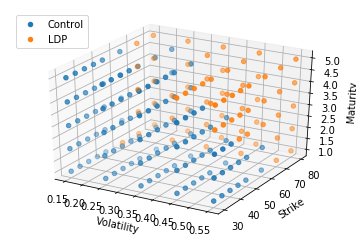
\includegraphics[width=0.4\textwidth]{content/reschap3/Figures/BS/compare1.png}
    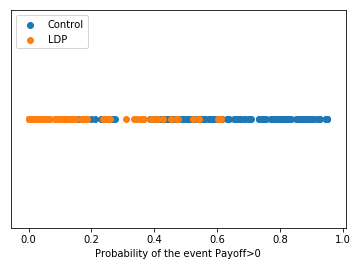
\includegraphics[width=0.4\textwidth]{content/reschap3/Figures/BS/compare2.png}
    \caption{Left:~Estimator with the highest variance reduction among antithetic, control and LDP estimators (Section~\ref{sec:BS_numerical_results}) for different values of~$\sigma$,~$K$,~$T$. Right:~Best performing estimator in terms of variance reduction among antithetic, control and LDP estimators (Section~\ref{sec:BS_numerical_results}) as a function of probability of a positive payoff (estimated using Monte-Carlo). Clearly, the LDP estimator performs best when the probability of exercising an option is low.
    }\label{fig:BSCompare}
\end{figure}
\begin{figure}[H]
    \centering
    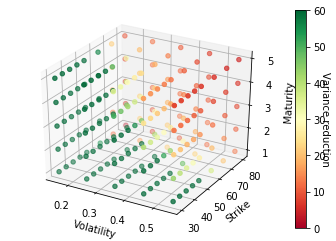
\includegraphics[width=0.4\textwidth]{content/reschap3/Figures/BS/control.png}
    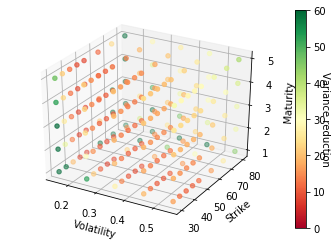
\includegraphics[width=0.4\textwidth]{content/reschap3/Figures/BS/ldp.png}
    \caption{Variance reduction of the control (left) and 
     the LDP (right) estimators}\label{fig:BSLDP}
\end{figure}

\begin{table}[H]
\centering
\begin{tabular}{lrrrr}
\toprule
 Strike~$K$ &  Antithetic &  Control &  LDP &  Probability of positive Payoff \\
\midrule
     30 &          64 &      769 &   53 &                            0.95 \\
     35 &          59 &      775 &   21 &                            0.95 \\
     40 &          31 &      744 &   10 &                             0.9 \\
     45 &          10 &      575 &  7.9 &                            0.75 \\
     50 &         3.8 &      336 &  8.6 &                             0.5 \\
     60 &         2.2 &       69 &   22 &                            0.11 \\
     70 &         2.0 &       16 &  123 &                           0.013 \\
     80 &         2.3 &      6.9 & 1445 &                          0.0011 \\
\bottomrule
\end{tabular}
\caption{Variance reduction for several estimators for Arithmetic Call options in Black-Scholes with~$S_0=50$,~$r=0.05$,~$\sigma = 0.25$ and~$T=1$.}\label{table:BSCompare}
\end{table}
%%%%%%%%%%%%%%%%%%%%%%%%%%%%%%%%%%%%%%%%%%%
%%%%%%%%%%%%%%%%%%%%%%%%%%%%%%%%%%%%%%%%%%%
\subsection{Numerical results for the Heston model}
\subsubsection{Asian option in Heston}
To compare variance reduction results in the Heston model, we look at Asian Geometric Call options, with payoffs of the form
\[
\left(\exp\left\{\frac{1}{T}\int_0^T X_t\D t\right\} - K\right)^+ = \left(S_0 \exp\left \{\frac{rT}{2}\int_0^T\frac{T-t}{T}\D X_t\right \} - K\right)^+,
\]
where~$x^+ = \max\{x,0\}$. 
We consider the following model parameters 
(realistic on Equity markets)
for the Heston model recalled in Section~\ref{sec:Heston}:
$$
S_0 = 50\,; \quad
r = 0.05\,; \quad
v_0 = 0.04\,; \quad
\rho = -0.5\,; \quad 
\kappa = 2\,; \quad
\theta = 0.09\,; \quad 
\xi = 0.2\,.
$$
To simulate the paths~$(X,V)$ on~$[0,T]$, 
we use a standard Euler-Maruyama scheme for~$X$, but use the scheme~\cite{Lord2009AModels} for the CIR process in the volatility, 
which is upward biased\footnote{There are many discretisation schemes for the Heston model. 
Since the objective of this chapter is not to study the effects of different schemes we satisfy ourselves with~\cite{Lord2009AModels}.}, however nevertheless converges strongly in~$L^1$ to the true process~$V$, which is enough for the purpose of pricing. For~$n\in\NN$,~$\Delta =\frac{T}{n}$ and the increments of the Brownian motion~$\{\Delta W_{i}^n\}_{i=0}^{n-1}$ the discretisation scheme over~$[0,T]$ for the variance process~$\{V_i^n\}_{i=0}^n$ reads:
\begin{equation*}
\left\{
\begin{array}{rcl}
\widetilde{V}_{0}^n & = & v_0>0\,, \\
\widetilde{V}_{i+1}^n & = & \widetilde{V}_{i}^n + \kappa \left(\theta - \widetilde{V}_{i}^{n,+}\right)\Delta + \xi \sqrt{\widetilde{V}_{i}^{n,+}}\Delta W_{i}^n, \quad \text{for all} \quad i\in\{0,\dots,n-1\}\,, \\
V_{i}^n & = & \widetilde{V}_{i}^{n,+}\,.
\end{array}
\right.
\end{equation*}
In what follows, we compare different LDP and MDP, with~$n=252$ trading days per year. 
All the results are computed for~$T=1$ using~$N_{\text{MC}}=500,000$ Monte-Carlo samples. 
We also consider an antithetic estimator and an LDP estimator derived assuming a deterministic volatility (denoted by BS).
Furthermore, since LDP-based deterministic changes of drift in the BS setting (or in cases where the final form of the optimisation problem is similar) are easy to compute, we also propose a \textit{fully adaptive} scheme based on the BS estimator: 
$$
h_t=\sum_{i=1}^{n} h^i_t \, \ind_{[(i-1)\Delta, i\Delta]}(t),
$$
where~$h^i_t$ is the best deterministic change of drift up to the~$i$-th discretisation step.\footnote{Fully adaptive schemes are computationally very heavy, therefore we only consider it in the Black-Scholes setting. 
The change of law is computed~$n \times N_{\text{MC}}$ times ($252 \times 5\mathrm{E}5 = 1.26\mathrm{E}8$ in our case).} %not sure I understand what the fully adaptive estimator is. Is it computed on each path up to each discretisation step? So~$$h_t=\sum_{i=1}^{n} h^i_t \, \ind_{[(i-1)\Delta, i\Delta)}(t),$$
We shall refer to \textit{deterministic} schemes
to mean changes of law with deterministic changes of drift and to \textit{adaptive} changes of drift 
for changes of law with drift of the form~$\int_0^\cdot \dot{h}_t\sqrt{V_t}\D t$.

%%%%%%%%%%%%%%%%%%%%%%%%%%%%%%%%%%
\subsubsection{LDP results in different settings}
We now look at the results of LDP-based estimators in \textit{small-noise}, \textit{small-time} and \textit{large-time} setting. Figure~\ref{fig:LDPvarianceRedu} indicates that the estimators derived
%in small-noise log-price
% and small-noise price have very similar variance reduction. On the other hand,
in small-time setting provide good results, but are outperformed by small-noise estimators. Although not apparent in the figure, looking at Table~\ref{tab:VarRedu}, the adaptive estimators provide slightly better results, as a matter of fact, they are notably better for small strikes. However, the computation time is also higher for adaptive estimators, which balances out the slight increase in variance reduction for higher strikes.
It thus seems that LDP adaptive estimators (in this case) imply a higher computational cost (given in Table~\ref{tab:CompTime}) which is not justified
by the variance reduction they can provide.
\begin{figure}[H]
    \centering
    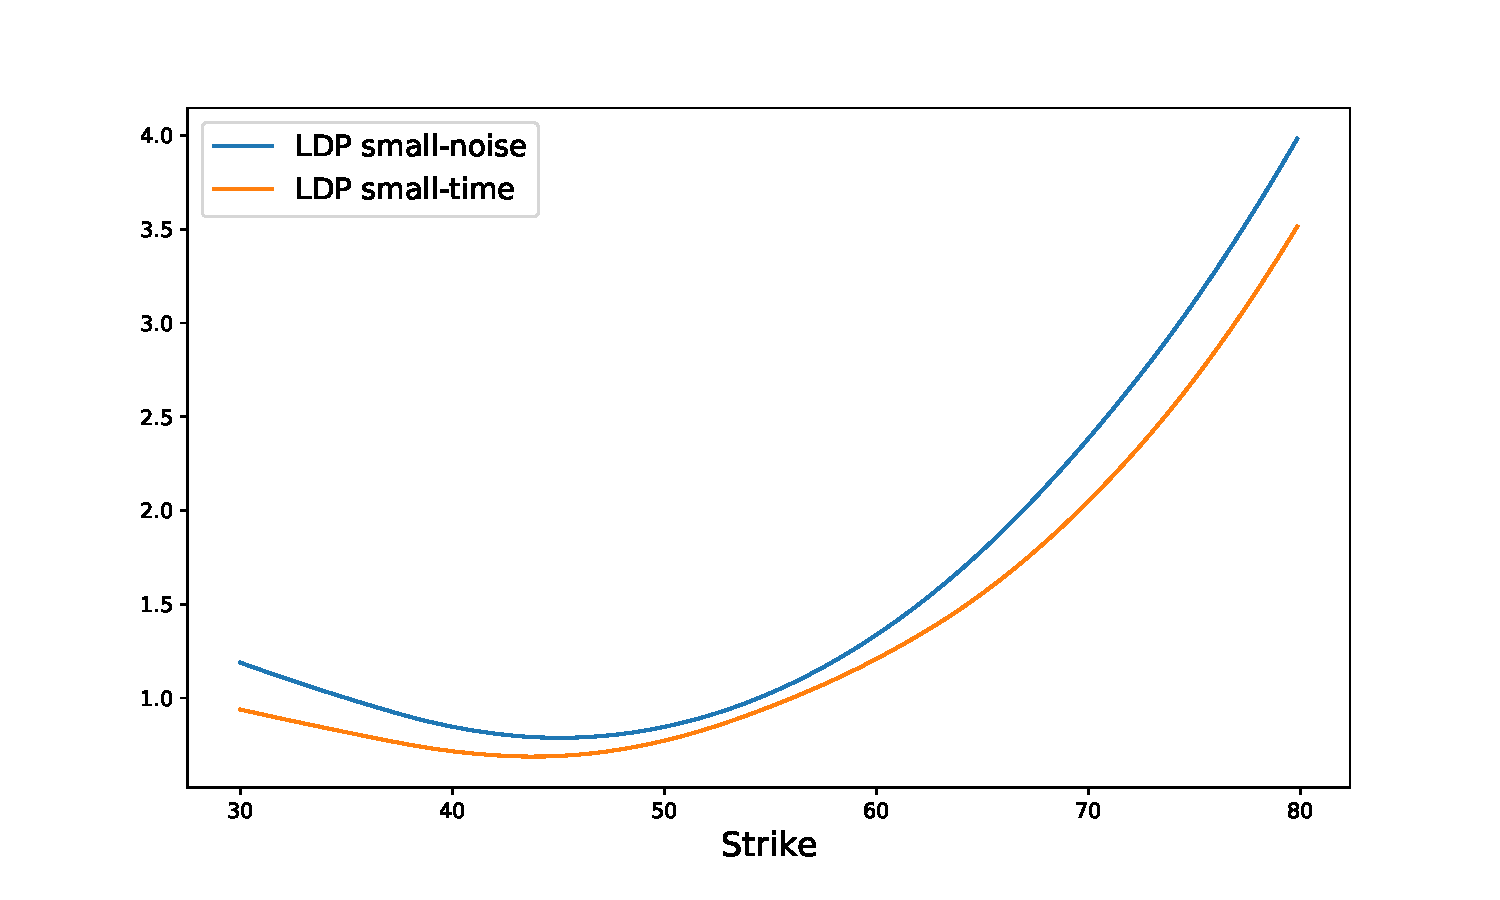
\includegraphics[width=0.495\textwidth, trim={2cm 0.5cm 2cm 1cm }]{content/reschap3/Figures/HESTON/compare-ldp-new.pdf}
    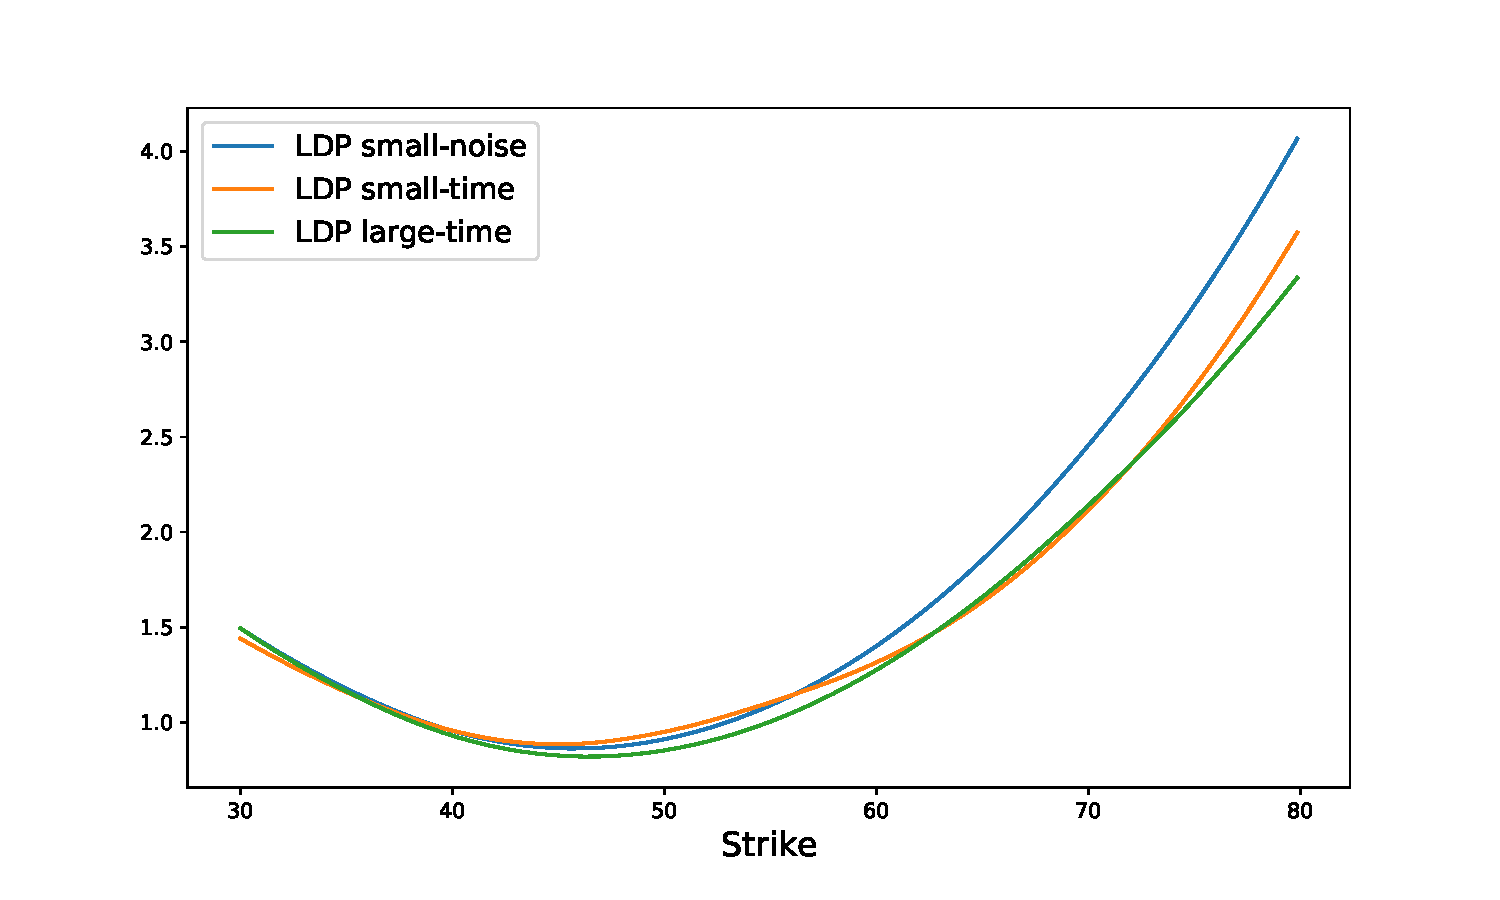
\includegraphics[width=0.495\textwidth, trim={2cm 0.5cm 2cm 1cm }]{content/reschap3/Figures/HESTON/compare-ldpada1-new.pdf}
    \caption{Variance reduction for LDP-based estimators in log-scale. \textit{Left}: deterministic change of drift. \textit{Right}: adaptive changes of drift.}\label{fig:LDPvarianceRedu}
\end{figure}

%%%%%%%%%%%%%%%%%%%%%%%%%%%%%%%%%%
\subsubsection{MDP results in different settings}

In the deterministic case, all considered estimators have similar variance reduction (see Figure~\ref{fig:MDPvarianceRedu}). 
To be more precise, the BS estimator has a very similar variance reduction or even slightly outperforms the MDP-based estimators (left plot of Figure~\ref{fig:MDPvarianceRedu}, where the lines are almost indistinguishable except for very high strikes, outside the `moderate' domain, which hence cause numerical problems). Therefore, in that aspect, MDP-based estimators do not justify their higher computational cost compared to the simple LDP-BS estimator. In the adaptive case, the BS estimator performs slightly better than before, whereas the MDP-based estimators significantly outperform their results from the deterministic case \textit{and} those of the BS estimator. Moreover, as it will be discussed in the next section, their variance reduction is in fact even close to that of the LDP-based estimators.
\begin{figure}[H]
    \centering
    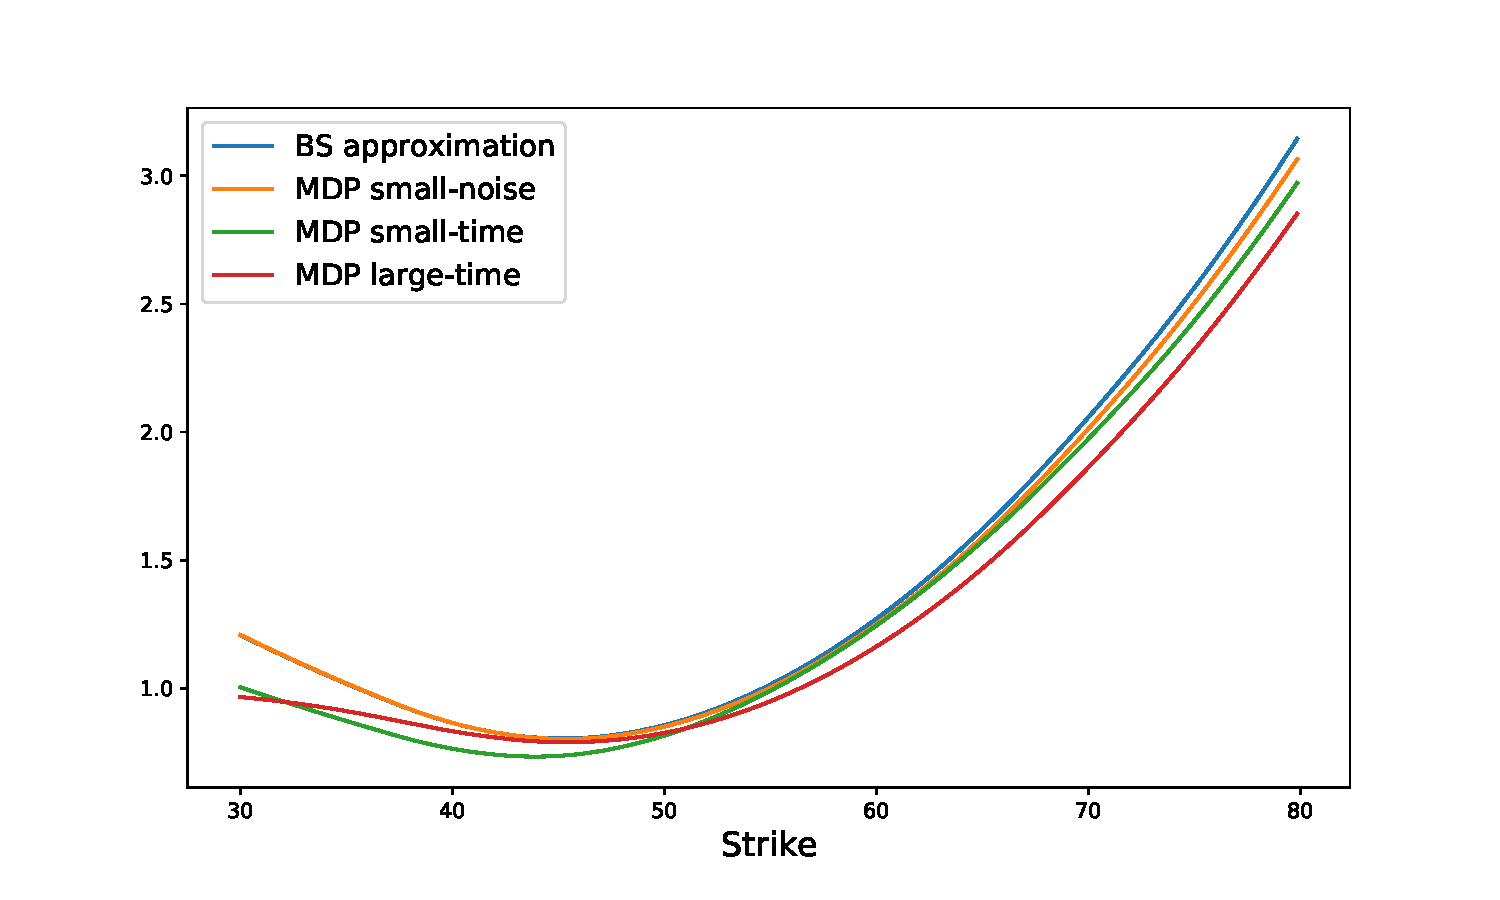
\includegraphics[width=0.495\textwidth, trim={2cm 0.5cm 2cm 1cm }]{content/reschap3/Figures/HESTON/compare-mdp-new.pdf}
    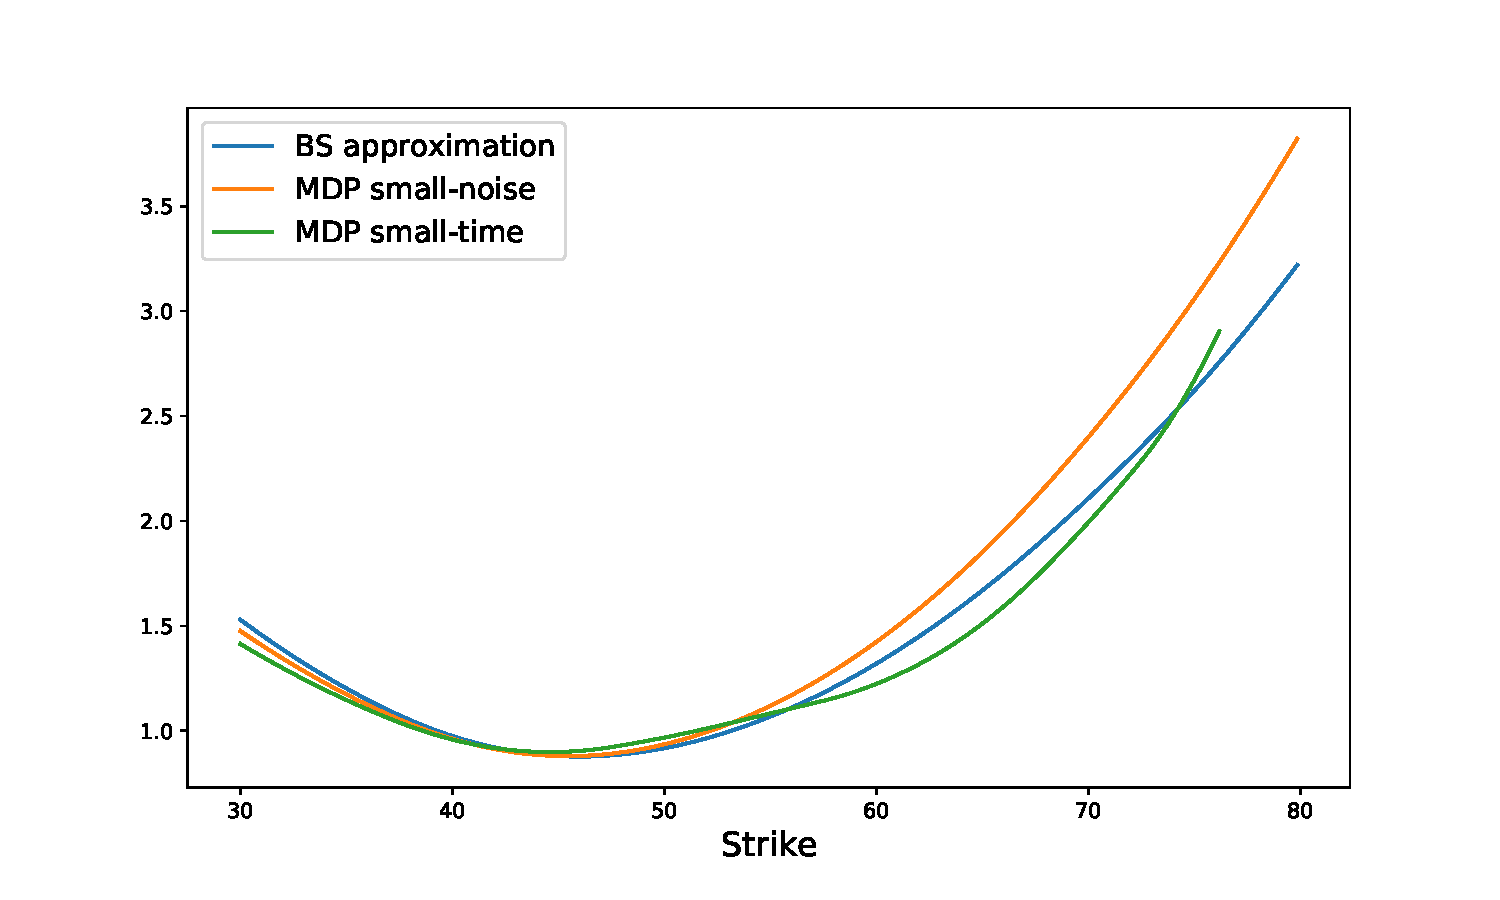
\includegraphics[width=0.495\textwidth, trim={2cm 0.5cm 2cm 1cm }]{content/reschap3/Figures/HESTON/compare-mdpada1-new.pdf}
    \caption{Variance reduction for MDP-based estimators for in log-scale. \textit{Left}: deterministic change of drift. \textit{Right}: adaptive changes of drift. Because of computational problems, the adaptive small-time MDP estimator was not computed correctly for strikes greater than~$75$. Nevertheless, it looks to be outperformed significantly by other MDP estimators.}\label{fig:MDPvarianceRedu}
\end{figure}

%%%%%%%%%%%%%%%%%%%%%%%%%%%%%%%%%%%%%%%%%%%%%%%%%%%
%%%%%%%%%%%%%%%%%%%%%%%%%%%%%%%%%%%%%%%%%%%%%%%%%%%
\subsubsection{Overall comparison}

Looking at Figure~\ref{ref:OverallVarRedu}, as expected the LDP small-noise adaptive estimators perform best, although MDP small-noise and large-time adaptive estimators are not far behind. 
As for the computation times, Table~\ref{tab:CompTime} indicates MDP estimators are on average about~$10\%$  and LDP estimators approximately~$15\%$ slower than the corresponding standard BS estimators. The fully adaptive BS estimator provides interesting results, especially for near-the-money strikes, where it performs much better than MDP and LDP estimators. 
Although the estimator is time-consuming, it can still provide a good balance between variance reduction and computation time for certain strikes (Tables~\ref{tab:VarRedu}-\ref{tab:VarComp}-\ref{tab:CompTime} and Figure~\ref{ref:OverallVarComp}).
In the following three tables and plots, we use the following short notations (within brackets their precise meanings, used in the graphs):

\begin{enumerate}[-]
    \item \textbf{Prob}: Probability of having a positive payoff.
    \item \textbf{LDPsn} (\textit{LDP small-noise}): Deterministic estimator based on LDP in small-noise log-price setting.
    \item \textbf{LDPsn A} (\textit{LDP small-noise adaptive}): Adaptive estimator based on LDP in small-noise log-price setting.
    \item \textbf{BS} (\textit{BS approximation}): Deterministic BS estimator.
    \item \textbf{BS A} (\textit{BS approximation adaptive}): Adaptive BS estimator.
    \item \textbf{MDPsn A} (\textit{MDP small-noise adaptive}): Adaptive estimator based on MDP in small-noise log-price setting.
    \item \textbf{BS A2} (\textit{BS fully adaptive}): Fully adaptive BS estimator.
    \item \textbf{Ant} (\textit{antithetic}): Antithetic estimator.
    \item \textbf{Classic}: Classic Monte-Carlo estimator.
\end{enumerate}

\begin{figure}[hbt!]
    \centering
    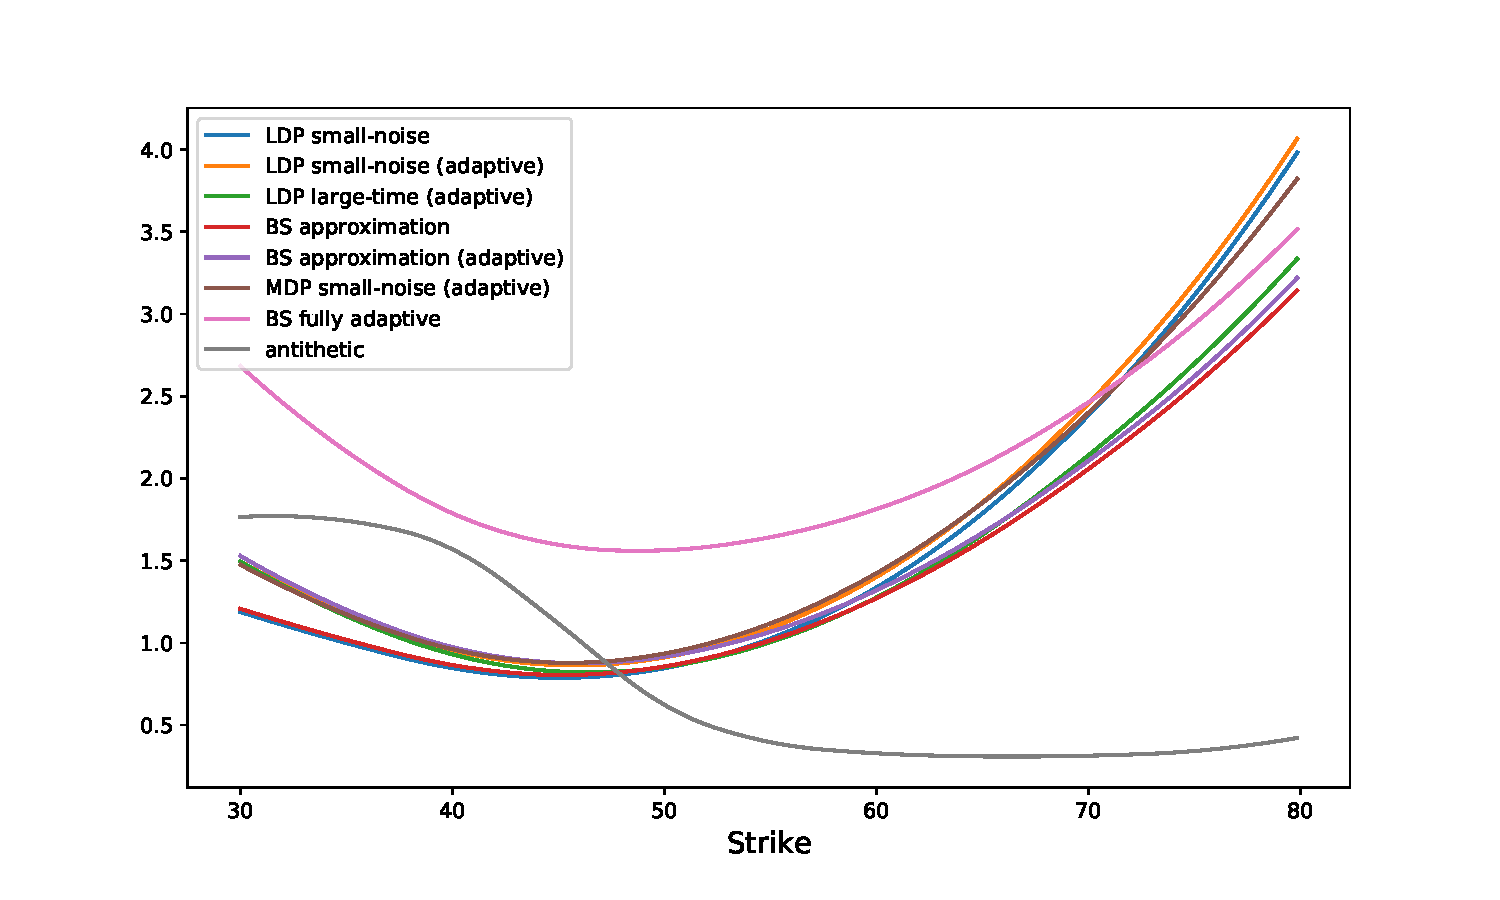
\includegraphics[scale=0.4]{content/reschap3/Figures/HESTON/compare-all-new.pdf}
    % 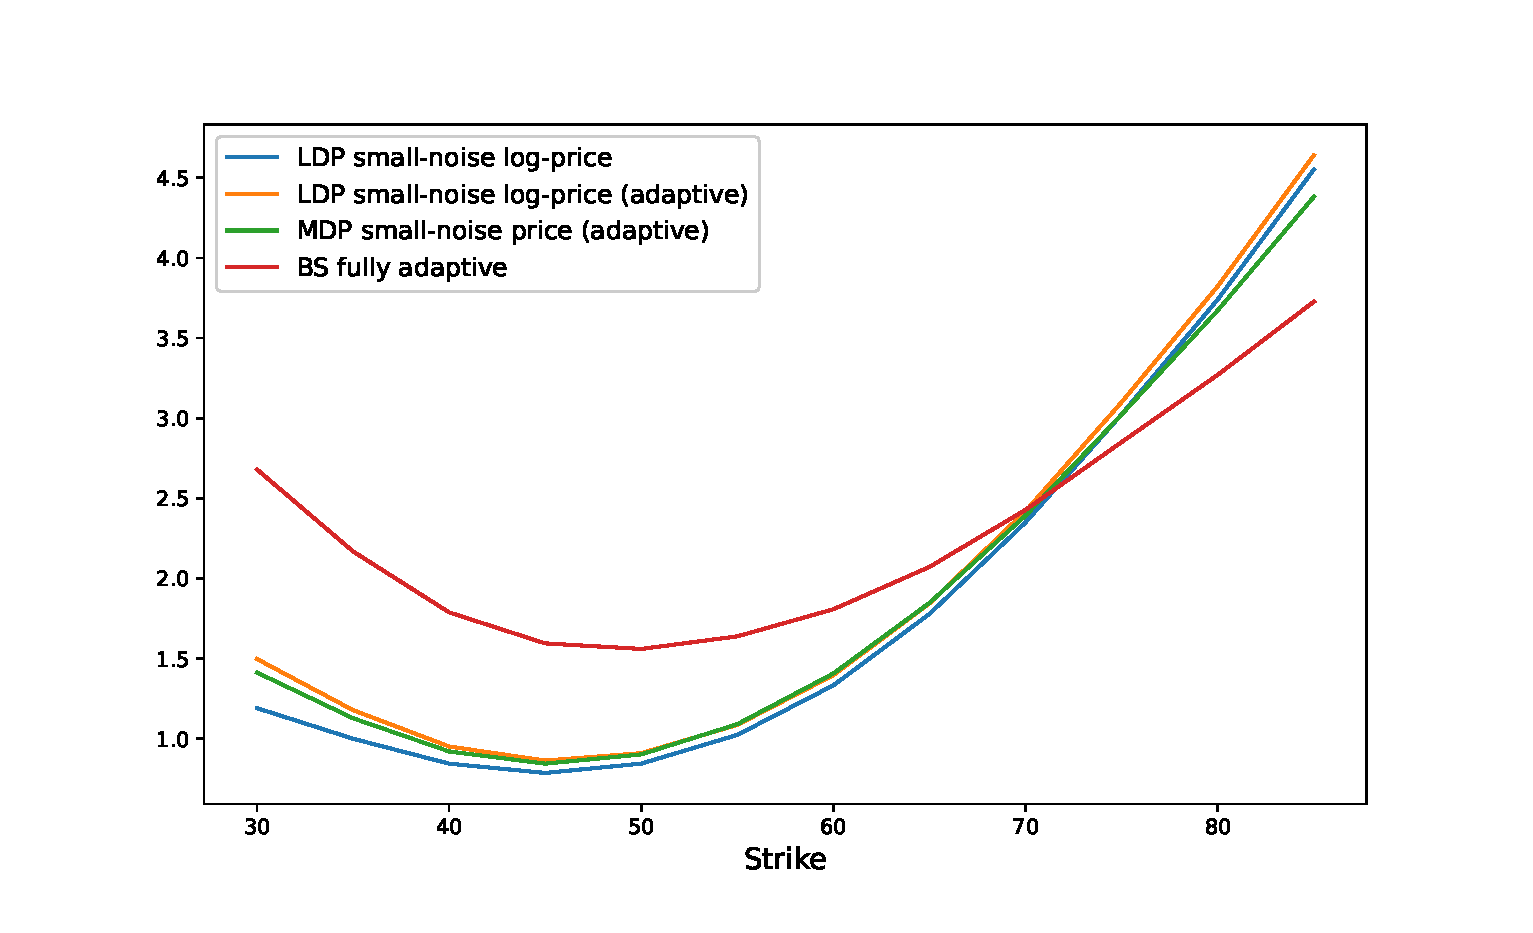
\includegraphics[width=0.495\textwidth, trim={2cm 0.5cm 2cm 1cm }]{HESTON/compare-sample.eps}
    \caption{Variance reduction for different estimators in log-scale. 
    The antithetic estimator offers almost no variance reduction for OTM options, because with high strikes very few paths end up in-the-money, thus reducing the effect of antithetic samples.}\label{ref:OverallVarRedu}
\end{figure}

\begin{figure}
    \centering
    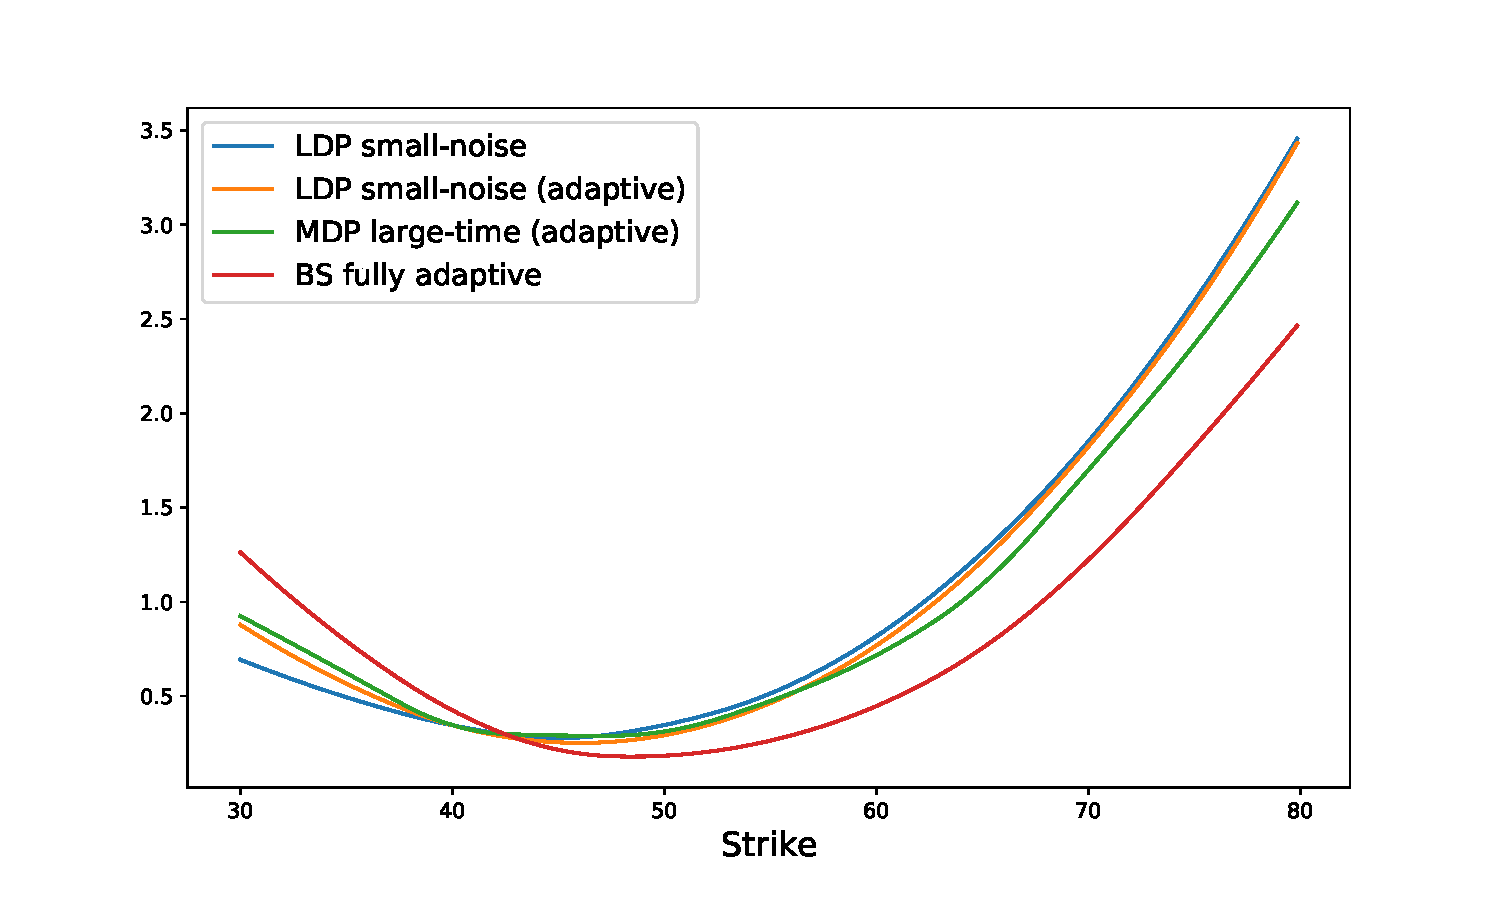
\includegraphics[scale=0.4]{content/reschap3/Figures/HESTON/compare-perf-new.pdf}
    \caption{Ratio of variance reduction over computation time for selected estimators in log-scale.}\label{ref:OverallVarComp}
\end{figure}

\begin{table}[H]
\centering
\begin{tabular}{lrrrrrrrr}
\toprule
Strike &   Prob. &  LDPsn &  LDPsn A &   BS &  BS A &  MDPsn A &  BS A2 &  Ant \\
\midrule
30 &    0.95 &     14 &       26 &   16 &    33 &           29  &    \textbf{470} &   58 \\
35 &    0.94 &    9.4 &       13 &   10 &    15 &           14  &    \textbf{150} &   55 \\
40 &     0.9 &    6.6 &      8.2 &  7.3 &   9.3 &          9.1  &     \textbf{60} &   36 \\
45 &    0.76 &    5.8 &      6.7 &  6.4 &   7.5 &          7.5  &     \textbf{39} &   13 \\
50 &    0.52 &    6.6 &      7.5 &  7.1 &   8.2 &          8.5  &     \textbf{36} &  4.2 \\
55 &    0.26 &     10 &       11 &   10 &    11 &           13  &     \textbf{43} &  2.5 \\
60 &   0.096 &     20 &       23 &   18 &    20 &           26  &     \textbf{64} &  2.1 \\
65 &   0.025 &     58 &       65 &   41 &    46 &           69  &    \textbf{120} &  2.0 \\
70 &   0.005 &    220 &      250 &  110 &   120 &          240  &    \textbf{280} &  1.9 \\
75 & 0.00078 &   1100 &     \textbf{1200} &  310 &   350 &          960 &    750 &  1.9 \\
80 &  0.0001 &   5700 &     \textbf{6800} &  860 &   990 &         4000 &   2000 &  1.7 \\
85 & 1.1e-05 &  35000 &    \textbf{43000} & 2400 &  2800 &        18000 &   5900 &  2.7 \\
\bottomrule
\end{tabular}
\bigskip
\caption{Variance reduction for different types of estimators and probability of positive payoff.}\label{tab:VarRedu}
\end{table}

\begin{table}[H]
\centering
\begin{tabular}{lrrrrrrrr}
\toprule
Strike &   Prob. &  LDPsn &  LDPsn A &  BS &  BS A &  MDPsn A &  BS A2 &  Ant \\
\midrule
30 &    0.95 &    3.3 &      4.0 & 3.2 &   5.6 &          4.6  &     \textbf{19} &  14.5 \\
35 &    0.94 &    2.3 &      2.0 & 2.2 &   2.9 &          2.4  &    5.0 &  \textbf{13.8} \\
40 &     0.9 &    1.5 &      1.3 & 1.4 &   1.5 &          1.4  &    2.7 &  \textbf{9.0} \\
45 &    0.76 &    1.4 &      1.1 & 1.2 &   1.4 &          1.3  &    1.9 &  \textbf{3.25} \\
50 &    0.52 &    1.6 &      1.1 & 1.3 &   1.2 &          1.2  &    \textbf{1.7} & 1.1 \\
55 &    0.26 &    \textbf{2.3} &      1.5 & 2.0 &   1.9  &      1.4 &    2.1 &  0.41 \\
60 &   0.096 &    \textbf{4.7} &      3.6 & 3.5 &   3.7  &      3.4 &    3.2 & 0.35 \\
65 &   0.025 &     \textbf{11} &      9.8 & 7.2 &   7.4 &           \textbf{11} &    6.0 & 0.33 \\
70 &   0.005 &     \textbf{48} &       33 &  16 &    21 &           31 &     16 & 0.32 \\
75 & 0.00078 &    \textbf{240} &      180 &  48 &    63 &          160 &     52 & 0.27 \\
80 &  0.0001 &   \textbf{1300} &      960 & 180 &   180 &          660 &    160 & 0.28 \\
85 & 1.1e-05 &   \textbf{7300} &     6600 & 490 &   500 &         3000 &   510 & 0.45 \\
\bottomrule
\end{tabular}
\bigskip
\caption{Ratio of variance reduction over computation time for different estimators.}\label{tab:VarComp}
\end{table}

\begin{table}[H]
\centering
\begin{tabular}{lrrrrrrrr}
\toprule
Strike &  Classic &  LDPsn &  LDPsn A &  BS &  BS A &  MDPsn A &  BS A2 &  Ant \\
\midrule
30 &       11 &     12 &       14 &  12 &    13 &           14  &     31 &   11 \\
35 &       11 &     11 &       14 &  12 &    13 &           13  &     36 &   11 \\
40 &       11 &     12 &       13 &  13 &    14 &           14  &     30 &   11 \\
45 &       11 &     11 &       13 &  13 &    13 &           13  &     28 &   11 \\
50 &       11 &     11 &       14 &  13 &    14 &           15  &     28 &   11 \\
55 &       11 &     12 &       15 &  12 &    13 &           15  &     28 &   11 \\
60 &       11 &     12 &       14 &  12 &    13 &           13  &     28 &   11 \\
65 &       11 &     12 &       14 &  13 &    13 &           13  &     27 &   11 \\
70 &       11 &     12 &       15 &  14 &    13 &           15  &     24 &   11 \\
75 &       11 &     12 &       14 &  14 &    13 &           13  &     21 &   11 \\
80 &       11 &     12 &       14 &  12 &    13 &           13  &     20 &   11 \\
85 &       11 &     12 &       14 &  12 &    13 &           13  &     19 &   11 \\
\bottomrule
\end{tabular}
\bigskip
\caption{Computation time (in seconds) for different estimators.}\label{tab:CompTime}
\end{table}

%%%%%%%%%%%%%%%%%%%%%%%%%%%%%%%%%%%%%%%%%%
\subsubsection{Variance swaps in Heston}
The methodology can also be applied to options with payoffs depending on volatility,
for example for options with payoffs of the form
$\int_0^T V_t \ind_{\{S_t\geq K\}}\D t$.
Consider~$T = 1$ and different strikes~$K>0$ under the Heston model with the same parameters as above. The results for different estimators are summarised in Table~\ref{tab:VarSwap}.
For small strikes, the LDP estimators based on the BS approximation are not performing well, which is not surprising since in the BS approximation the payoff of the option in question is almost constant for small strikes. On the other hand, LDP and MDP give good results. We also notice a clear difference in favour of non-adaptive changes of drift.
For high strikes, we have the same behaviour as before: adaptive MDP estimators give intermediate results between LDP (performing best) and BS. At this stage though, we do not have a clear explanation for the observed differences in the performance of non-adaptive and adaptive changes of drift for different strikes. Further research is required to understand the underlying dynamics better.

\begin{table}[H]
\centering
\begin{tabular}{lrrrrrrr}
\toprule
Strike &  LDPsn &  LDPsn A &  MDPsn &  MDPsn A &  BS &  BS A &  Ant \\
\midrule
10  &    \textbf{220} &       43 &    190 &       44 & 1.0 &   1.0 &   45 \\
20  &    \textbf{160} &       38 &    140 &       38 & 1.0 &   1.0 &   46 \\
30  &    8.2 &      6.3 &    8.6 &      6.5 & 1.0 &   1.0 &   \textbf{14} \\
40  &    1.1 &      1.1 &    1.1 &      1.1 &   1 &     1 &  \textbf{2.5} \\
45  &   0.86 &     0.85 &   0.88 &     0.87 & 1.0 &   1.0 &  \textbf{2.9} \\
50  &   0.96 &     0.96 &   0.86 &     0.76 & 1.0 &   1.0 &   \textbf{12} \\
55  &    2.4 &      2.5 &    2.6 &      2.4 & 1.8 &   1.9 &  \textbf{6.8} \\
60  &    3.1 &      3.3 &    \textbf{4.4} &      3.0 & 3.8 &   4.1 &  3.2 \\
70  &    8.4 &  \textbf{9.1} &    7.4 &      6.9 & 6.4 &   7.0 &  2.1 \\
80  &     16 &  19 &     15 &       \textbf{22} &  11 &    11 &  2.0 \\
90  &     56 &  \textbf{68} &     26 &       54 &  17 &    19 &  1.9 \\
100 &    200 &      \textbf{240} &     36 &      190 &  42 &    54 &  2.3 \\
\bottomrule
\end{tabular}
\caption{Variance reduction for different estimators.}\label{tab:VarSwap}
\end{table}

